\setcounter{section}{0}

\section{Introducción}
Nuestro principal objetivo en este apartado será predecir a través de los distintos modelos disponibles en las librerias de $\textsf{R}$. Para ello vamos a trabajar con una única serie durante todo el apartado ($\verb!accidentes!$), que se corresponde al número de accidentes de tráfico ocurridos mensualmente en Ontario en el periodo 1960-1974 \cite{datamarket}.

Para poder comparar entre todas las predicciones vamos a seguir el enfoque habitual del \textit{machine learning}, es decir, vamos a dividir nuestros datos en un conjunto de \textit{training} ($\verb!acc.train!$) que comprende los años 1960-1973 y en otro de \textit{test} ($\verb!acc.test!$) que comprende el año 1974. En el conjunto de \textit{training} vamos a entrenar a nuestro modelo y en el de \textit{test} le vamos a evaluar.

En la Figura \ref{accidentes} se puede apreciar como nuestra serie parece mostrar una pequeña tendencia creciente y una estacionalidad anual bastante marcada presentando picos en los meses de verano y en los correspondientes a las fechas navideñas, cosa que tiene sentido ya que es en estos periodos cuando la gente viaja más y por lo tanto hay más accidentes.
\begin{figure}
    \centering
    \centerline{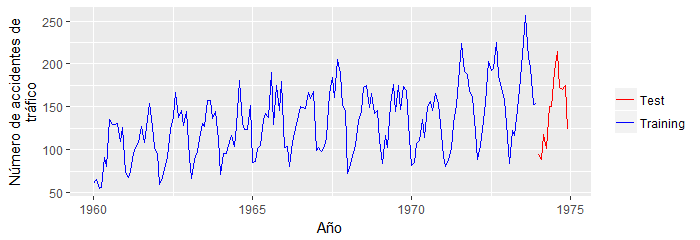
\includegraphics[scale = 0.7]{Images/Modelizacion/31.png}}
    \caption{Accidentes de tráfico ocurridos en Ontario en el periodo 1960-1975}
    \label{accidentes}
\end{figure}

\section{Forecast Package}
Esta librería está conformada por métodos orientados al análisis de series temporales univariantes, ya sea desde un punto de vista más clásico o desde uno más orientado a modelos del tipo ARIMA. Además incluye también algunos modelos de predicción algo más avanzados \cite{forecast}.

Esta vez vamos a utilizar la librería $\verb!rdatamarket!$ para importar a través de una API los datos en formato $\verb!zoo!$ directamente de la web de \textit{datamarket} \cite{datamarket}.

Esta librería es capaz de trabajar con cualquier tipo de objeto temporal pero personalmente recomiendo $\verb!ts!$ ya que en ocasiones se apoya en métodos de la librería $\verb!stats!$ para construir los distintos modelos. Aun así, como ya hemos visto en el apartado anterior, no suele haber problemas entre conversiones $\verb!ts!$ y $\verb!zoo!$. El código correspondiente a esta libreria se muestra en el Anexo III.

\subsection{Preprocesado}
En ocasiones nos puede resultar útil encontrar los periodos estacionales dominantes en nuestra serie, para ello podemos recurrir a $\verb!findfrequency()!$, un método que automáticamente nos devolverá el periodo estacional de nuestra serie, en nuestro caso es 12 (se presentan periodos cada 12 meses, es decir, cada año).

Un método muy útil para estudiar la estacionalidad es $\verb!seasonplot()!$. Con él vamos a poder representar gráficamente cada año (periodo estacional) por separado y comparar cómo evoluciona la estacionalidad a medida que pasa el tiempo. Su sintaxis es la siguiente:
\begin{Verbatim}[fontsize=\footnotesize]
seasonplot(x, s, …)
\end{Verbatim}

En el que $\verb!x!$ es la serie temporal a representar y $\verb!s!$ el periodo estacional. Una opción es introducir al argumento $\verb!s!$ la función $\verb!findfrequency()!$ aplicada a nuestra serie para que automáticamente utilice este periodo estacional. En la Figura \ref{season} se muestra el gráfico originado por este método correspondiente a nuestra serie $\verb!acc.train!$. En él se puede apreciar como el menor número de accidentes se registran a principio de año y este se va incrementando hasta que alcanza su máximo en los meses de verano, después disminuye en comparación con la primera mitad del año pero sigue mostrando valores altos en los últimos meses del año.
\begin{figure}
    \centering
    \centerline{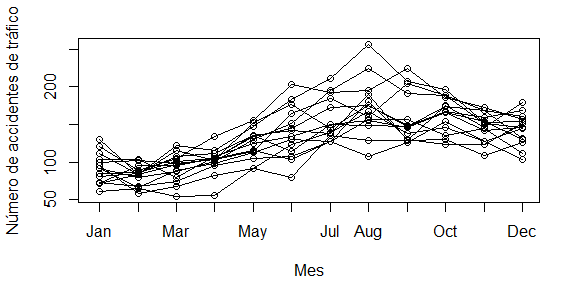
\includegraphics[scale = 0.7]{Images/Modelizacion/32.png}}
    \caption{Representación anual de la estacionalidad de la serie}
    \label{season}
\end{figure}

Vamos a descomponer nuestra serie con el método $\verb!decompose!$ de la librería $\verb!stats!$ y vamos a guardar el resultado en $\verb!acc.train.decomp!$. A través de los métodos $\verb!seasonal()!$, $\verb!trendcycle()!$ y $\verb!remainder()!$ vamos a poder extraer cada una de las componentes sin necesidad de hacer \textit{subsetting} del objeto generado por $\verb!decompose!$. Hemos supuesto que nuestra serie es multiplicativa ya que parece que el nivel estacional varía con el tiempo. En la Figura \ref{descompose} se muestra el resultado de esta descomposición.
\begin{figure} [t]
\begin{subfigure}{.5\textwidth}
  \centering
  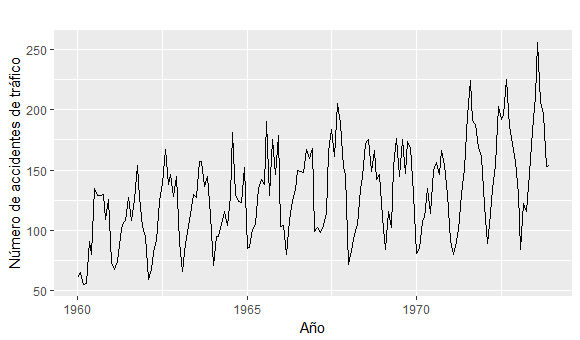
\includegraphics[width=.8\linewidth]{Images/Modelizacion/33-serie.png}
  \caption{Serie original}
  \label{fig:sfig1}
\end{subfigure}
\begin{subfigure}{.5\textwidth}
  \centering
  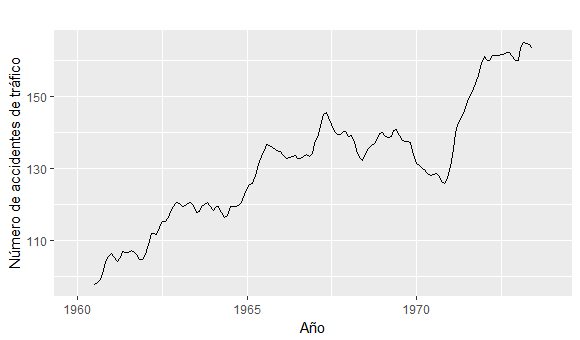
\includegraphics[width=.8\linewidth]{Images/Modelizacion/33-tend.png}
  \caption{Tendencia}
  \label{fig:sfig2}
\end{subfigure}
\begin{subfigure}{.5\textwidth}
  \centering
  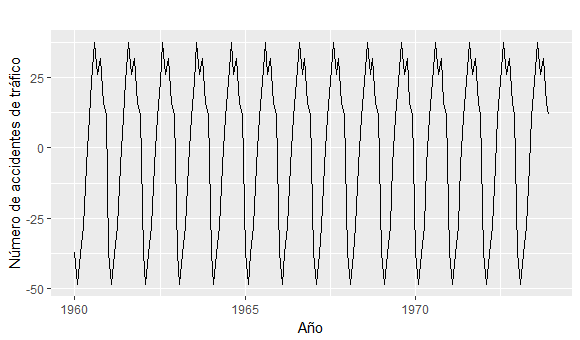
\includegraphics[width=.8\linewidth]{Images/Modelizacion/33-season.png}
  \caption{Estacionalidad}
  \label{fig:sfig1}
\end{subfigure}
\begin{subfigure}{.5\textwidth}
  \centering
  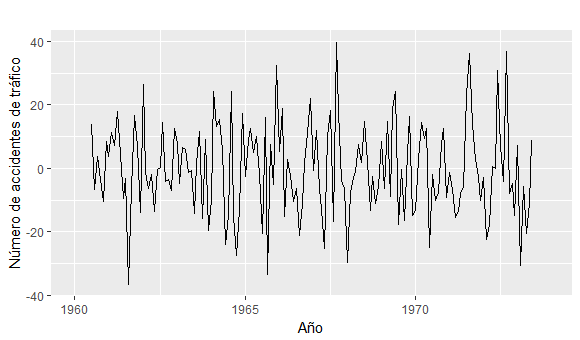
\includegraphics[width=.8\linewidth]{Images/Modelizacion/33-irre.png}
  \caption{Irregular}
  \label{fig:sfig2}
\end{subfigure}
\caption{Descomposición de la serie \PVerb{acc.train}}
\label{descompose}
\end{figure}

Para ver si realmente esta descomposición recoge todos los aspectos deterministas de la serie vamos a estudiar los residuos a través del método $\verb!Box.test!$ de la librería $\verb!stats!$. Este método implementa el test de Ljung-Box a nuestros residuos para contrastar la hipótesis nula de independencia entre observaciones. Obtenemos un p-valor de 0.7658 por lo que parece que esta descomposición recoge una parte importante de los patrones deterministas del proceso que genera nuestra serie ya que la componente aleatoria es ruido.

En la Figura \ref{descompose} se puede apreciar como la componente estacional se mantiene constante a lo largo del tiempo por lo que podría tener sentido eliminarla de la serie. Para ello recurrimos a $\verb!seasadj()!$. El resultado tras aplicar este método se muestra en la Figura \ref{deses}.
\begin{figure}
    \centering
    \centerline{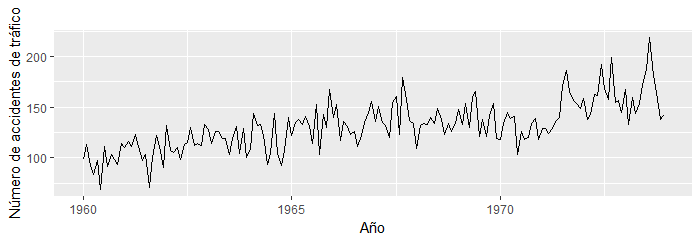
\includegraphics[scale = 0.7]{Images/Modelizacion/34.png}}
    \caption{Serie desestacionalizada}
    \label{deses}
\end{figure}

En ocasiones es muy importante saber si una serie es estacionaria o no, para ello se suelen recurrir a distintos test estadísticos de la raíz unitaria. En esta librería recomiendo el método $\verb!ndiffs()!$ con el cual se obtiene el número de diferenciaciones a aplicar a nuestra serie para que sea estacionaria. Si la salida es 0 significa que nuestra serie es estacionaria, en caso contrario no lo es. Su sintaxis es la siguiente:
\begin{Verbatim}[fontsize=\footnotesize]
ndiffs(x, alpha = 0.05, test = c("kpss", "adf", "pp"), max.d = 2)
\end{Verbatim}

Este método devuelve el número de veces que se ha tenido que diferenciar nuestra serie para asegurar la hipótesis de estacionariedad del test especificado a través de $\verb!test!$ a un nivel de significación introducido en $\verb!alpha!$. Nosotros usaremos el test aumentado de Dickey Fuller (ADF). Obtenemos una salida de 0 por lo que parece que no es necesario diferenciar la serie para trabajar bajo estacionariedad.

Al igual que en otras librerías es posible estudiar más en profundidad la tendencia a partir del método $\verb!ma()!$ encargado de aplicar un suavizado de medias móviles. En este caso tiene sentido suavizar la serie con un orden 12 para conseguir así sumarizar los datos anualmente eliminando la influencia de la estacionalidad, pudiéndose apreciar de forma más clara la evolución general de la serie.

\subsection{Modelos ingenuos}
El preprocesado de los datos temporales es importante pero como bien se puede apreciar en su propio nombre ($\verb!forecast!$) esta librería se centra en la predicción a través de modelos temporales. Estos modelos tienen sus propios métodos capaces de aportarnos información relevante para el correcto ajuste y predicción del modelo aplicado. Comenzaremos aplicando y estudiando los resultados de algunos modelos de predicción más sencillos.

Estos modelos sencillos o ingenuos se utilizan para trabajar bajo el principio de parsimonia. Bajo este principio conseguimos controlar la relación esfuerzo-resultado, evitando así destinar muchos recursos al ajuste de modelos complejos que apenas mejoran las predicciones de uno ingenuo.

El primer modelo ingenuo es el provisto por el método $\verb!meanf()!$ y consiste en simplemente predecir los valores de la serie a partir de su media. Su sintaxis es la siguiente:
\begin{Verbatim}[fontsize=\footnotesize]
meanf(y, h, level = c(80, 95), …)
\end{Verbatim}

\noindent donde $\verb!y!$ es un vector numérico o en nuestro caso una serie temporal, $\verb!h!$ es el número de periodos que deseamos predecir y $\verb!level!$ es el nivel de confianza de las predicciones realizadas. El objeto generado es de la clase $\verb!forecast!$ y nos aporta una gran cantidad de información útil para realizar diagnósticos de nuestro modelo (predicciones, residuales, serie original, etc…).

A continuación se muestra como ajustar un modelo ingenuo de estas características a la serie $\verb!acc.train!$ que se encargue de predecir los valores para el año 1974:

\begin{Verbatim}[fontsize=\footnotesize, numbers = left]
model <- meanf(acc.train, h = 12)
autoplot(model)
\end{Verbatim}

En la Figura \ref{meanf_1} generada por el código anterior se muestra la serie utilizada para entrenar al modelo y los resultados de la predicción. En este caso la predicción para el año 1974 es una línea recta ya que estamos utilizando únicamente la media. La franja azul clara representa el intervalo de confianza a un nivel del 95$\%$ y la más oscura al 80$\%$. La Figura \ref{comp} nos permite comparar gráficamente la predicción con los valores reales.
\begin{figure}
    \centering
    \centerline{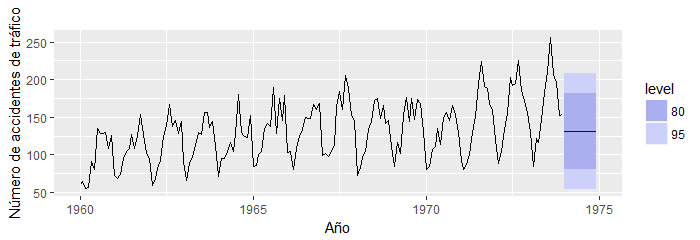
\includegraphics[scale = 0.7]{Images/Modelizacion/35.png}}
    \caption{Predicción del modelo correspondiente a \PVerb{meanf()}}
    \label{meanf_1}
\end{figure}

Inspeccionar gráficamente el ajuste del modelo no es siempre la mejor opción ya que en muchas ocasiones necesitaremos medidas más objetivas para, por ejemplo, comparar entre modelos. Esta librería incorpora un método muy útil conocido como $\verb!accuracy()!$. Su sintaxis es la siguiente:
\begin{Verbatim}[fontsize=\footnotesize]
accuracy(f, x, …)
\end{Verbatim}

A través del argumento $\verb!f!$ se introduce el modelo a evaluar almacenado en un objeto de clase $\verb!forecast!$. El argumento $\verb!x!$ es opcional, en él se introduce el conjunto de test en caso de que se disponga de uno. En nuestro caso vamos a pasar el método $\verb!accuracy()!$ a nuestro modelo \PVerb{model} y al conjunto de \textit{test} $\verb!acc.test!$. La salida resultante es la siguiente:
\begin{Verbatim}[fontsize=\footnotesize]
                       ME     RMSE      MAE        MPE
Training set 5.392491e-15 38.73302 31.48058 -10.085477
Test set     1.439286e+01 41.43521 36.28770   2.639993
                     MAPE     MASE      ACF1 Theil's U
                 27.71539 1.774836 0.7359523        NA
                 25.15689 2.045855 0.6310518  1.205019
\end{Verbatim}

Estamos obteniendo varias medidas de precisión tanto para el conjunto de \textit{training} como para el de \textit{test}. Nosotros nos centraremos en las dos siguientes:

\begin{description}
  \item[$\bullet$ RMSE:]Raíz del error cuadrático medio.
    \begin{equation}
    RMSE = \sqrt{\frac{1}{T} \sum_{i = 1}^{n}(Y_i - \widehat{Y}_i)^2}
    \end{equation}
  \item[$\bullet$ MAE:]Error medio absoluto.
  \begin{equation}
    MAE = \frac{1}{T} \sum_{i = 1}^{n} \lvert Y_i - \widehat{Y}_i \lvert
  \end{equation}
\end{description}

La MAE es muy común en las distintas competiciones de \textit{Data Science} que se realizan en Internet.

En nuestro modelo estamos obteniendo un RMSE y un MAE para el conjunto de \textit{training} de 38.73302 y 31.48058, respectivamente. Para el conjunto de \textit{test} obtenemos 41.43521 y 36.28770. En ambos conjuntos obtenemos errores similares (siendo mayores los del \textit{test}) lo cual es una buena señal. El MAE es fácilmente interpretable: en este caso significa que estamos errando en 36 accidentes mortales en promedio en nuestras predicciones.

Otro método muy útil incluido en esta librería es $\verb!checkresiduals()!$. Con él vamos a poder estudiar los residuos de los modelos ajustados ya que nos va a ofrecer su gráfico, su correlograma, su histograma y un test estadístico para contrastar la significatividad de las autocorrelaciones. Su sintaxis es la siguiente:
\begin{Verbatim}[fontsize=\footnotesize]
checkresiduals(object, lag, test, ...)
\end{Verbatim}

A través del argumento $\verb!object!$ vamos a introducir el modelo a evaluar, $\verb!lag!$ fija los rezagos a utilizar en el test estadístico y $\verb!test!$ el propio test que puede ser el de Ljung-Box o el de Breusch-Godfrey. Por defecto el método selecciona automáticamente el test de Breusch-Godfrey si el modelo a evaluar es de regresión, en caso contrario utiliza el de Ljung-Box.

En el caso de nuestro modelo ingenuo estamos obteniendo un p-valor para el test de Ljung-Box de prácticamente cero por lo que parece haber aún relaciones y patrones en los residuos.  Esto es algo lógico ya que la media es incapaz de recoger ningún patrón importante de los datos. Los gráficos resultantes se muestran en la Figura \ref{checkresiduals}.
\begin{figure}
    \centering
    \centerline{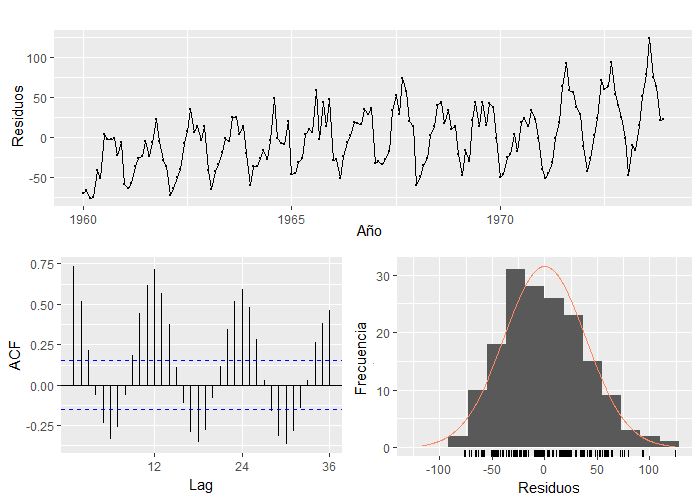
\includegraphics[scale = 0.7]{Images/Modelizacion/37.png}}
    \caption{Resultado del método \PVerb{checkresiduals()}}
    \label{checkresiduals}
\end{figure}

Es posible también utilizar el último valor observado para predecir los nuevos valores de la serie, el método $\verb!naive()!$ se encarga de implementar esto. La sintaxis es idéntica a la del método anterior y los resultados también, solo que en este caso la línea formada por los valores predichos está desplazada hacia arriba (el último valor de la serie es mayor que la media). Este resultado se muestra en la Figura \ref{comp}.

Obtenemos un RMSE y un MAE en el conjunto de \textit{test} de 39.73873 y 33.8333, respectivamente. Son unos resultados muy similares a los obtenidos por $\verb!meanf()!$ por lo que apenas hay diferencias entre ambos modelos. En este caso los residuos también parecen mostrar de forma significativa autocorrelaciones.

A través del método $\verb!rwf()!$ es posible ajustar una variante del modelo ingenuo provisto por $\verb!naive()!$ conocido como caminata aleatoria con deriva. Teóricamente se define como:
\begin{equation}
    Y_t = \delta + Y_{t - 1} + a_t
\end{equation}

\noindent por lo que realizaremos la predicción de $Y_{t + h}$ a partir de:
\begin{equation}
    \widehat{Y}_{t + h} = \delta h + \widehat{Y}_{t + h - 1}
\end{equation}

La deriva $\delta$ refleja el cambio medio de la serie a lo largo del tiempo y se calcula de la siguiente manera:
\begin{equation}
    \delta = \bigg( \frac{Y_T - Y_1}{T - 1} \bigg)
\end{equation}

Para incluir esta deriva es necesario pasar al argumento $\verb!drift!$ el valor de $\verb!TRUE!$, en caso contrario obtendremos los mismos resultados que con $\verb!naive()!$. En la Figura \ref{comp} se puede apreciar como en este caso las predicciones no forman una línea totalmente horizontal sino que presentan una pequeña pendiente gracias a la inclusión de la deriva. Obtenemos unas medidas de precisión prácticamente idénticas al modelo sin deriva y unos residuos correlacionados entre sí. Todo esto es lógico ya que la inclusión de la deriva no supone un mejor ajuste, nos falta algo a tener en cuenta en el modelo para lograr ajustes aceptables.

Como bien hemos comentado, esta serie muestra una componente estacional muy marcada por lo que una opción sería ajustar un modelo que predijese de acuerdo a los valores estacionales del periodo anterior, en este caso del año anterior. Esto es lo que ofrece $\verb!snaives()!$ que en vez de predecir con el valor inmediatamente anterior predice con el correspondiente al periodo estacional anterior, por ejemplo si queremos predecir el valor de nuestra serie en julio de 1974 este recurrirá al valor en julio de 1973. Más formalmente se define como:
\begin{equation}
    Y_t = Y_{t - M} + a_t
\end{equation}

\noindent siendo M el periodo estacional presente en la serie, en nuestro caso 12. En la Figura \ref{snaives} se observa como efectivamente lo único que hemos hecho ha sido predecir el año 1974 a partir del 1973. Aunque este método parece sencillo obtenemos un RMSE y un MAE de 25.98237 y 22.58333 respectivamente. Esto significa que estamos consiguiendo obtener un ajuste relativamente bueno, esto se debe a que esta serie parece mostrar un comportamiento estacional bastante estable en los últimos años estudiados. Sin embargo no es suficiente ya que el test de Ljung-Bbox nos dice que aún existen correlaciones entre los residuos, necesitamos algo más avanzado.
\begin{figure}
    \centering
    \centerline{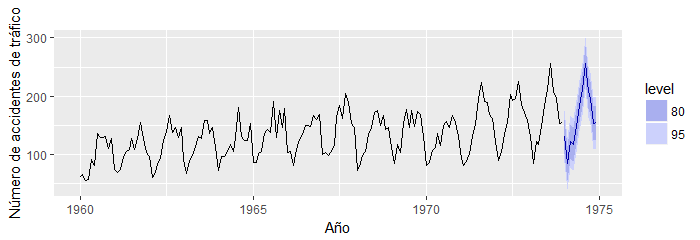
\includegraphics[scale = 0.7]{Images/Modelizacion/310.png}}
    \caption{Predicción del modelo correspondiente a \PVerb{snaives()}}
    \label{snaives}
\end{figure}

\begin{figure}
    \centering
    \centerline{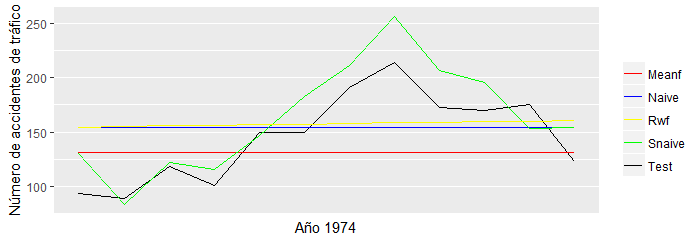
\includegraphics[scale = 0.7]{Images/Modelizacion/311.png}}
    \caption{Comparación de los modelos ingenuos con el \textit{test}}
    \label{comp}
\end{figure}

\subsection{Modelo lineal}
A continuación vamos a manejar algunos modelos más completos a fin de conseguir un mejor ajuste. Comenzaremos ajustando un modelo de regresión lineal con la tendencia y la estacionalidad como variables independientes:
\begin{equation}
    Y_{t} = \beta_0 + \beta_1 t + \sum_{i = 2}^{M} \lambda_i d_i
\end{equation}

\noindent donde $d_i$ son variables dummy que toman el valor 1 cuando $i = m$ con $m \neq 1$ siendo $m$ el periodo al que corresponde $Y_t$. Los coeficientes $\lambda_i$ se interpretan como el cambio medio correspondiente al periodo estacional $i$. Para ajustar este tipo de modelos recurriremos al método $\verb!tslm()!$. Este método funciona de la misma manera que $\verb!lm()!$, solo que nos permite añadir y calcular las variables independientes correspondientes a la tendencia y a la estacionalidad de forma mucho más sencilla. A continuación se muestra el código para ajustar este modelo a nuestros datos pudiendo así predecir un año:
\begin{Verbatim}[fontsize=\footnotesize, numbers = left]
model <- tslm(acc.train ~ trend + season)
pred <- forecast(model, h = 12)
\end{Verbatim}

La sintaxis seguida es la utilizada en $\verb!lm()!$, es decir, estamos ajustando un modelo de regresión con $\verb!acc.train!$ como variable dependiente y $\verb!trend!$ y $\verb!season!$ como independientes (estas variables son calculadas internamente por el propio método). En este caso el método $\verb!tslm()!$ no nos generará un objeto $\verb!forecast!$ sino $\verb!lm!$ por lo que necesitamos transformarlo mediante $\verb!forecast()!$ introduciendo como argumentos el modelo y el número de observaciones a predecir.

A través del \textit{subsetting} $\verb!$coefficients!$ es posible acceder a los coeficientes de nuestro modelo. El modelo final ajustado es el siguiente:
\begin{equation}
    \widehat{Y}_{t} = 63.75 + 0.35 t - 9.99 d_2 - 0.06 d_3 + 8.72 d_4 + ... + 47.88 d_{12}
\end{equation}

El resultado de la predicción se muestra en la Figura \ref{tslm}. Estamos obteniendo un MAE de 19.44597 que es el mejor hasta el momento, sin embargo seguimos teniendo correlaciones entre los residuos por lo que parece que este modelo no acaba de recoger todas las relaciones presentes en nuestra serie.
\begin{figure}
    \centering
    \centerline{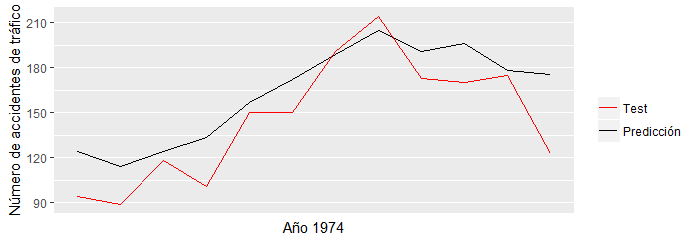
\includegraphics[scale = 0.7]{Images/Modelizacion/312.png}}
    \caption{Comparación de las predicciones realizadas por \PVerb{tslm()} con el \textit{test}}
    \label{tslm}
\end{figure}

\subsection{Triple suavizado exponencial}
Los modelos de suavizado exponencial pueden parecer simples a primera vista pero en ocasiones consiguen realizar predicciones bastante acertadas. Nuestra serie presenta tendencia y estacionalidad por lo que es posible modelizarla a través de un triple suavizado exponencial o Holt-Winters, con coeficientes $\alpha$, $\beta$ y $\gamma$. La idea es aplicar un suavizado exponencial ponderado a la componente estacional, al nivel y a la tendencia

Este modelo está compuesto por tres ecuaciones de suavizado y una de predicción. Estas tres ecuaciones estiman individualmente el nivel $l_t$ (el valor suavizado de la serie), la tendencia $b_t$ y la estacionalidad $S_t$. Estos tres componentes se relacionan en la ecuación de predicción para obtener el valor estimado. A continuación se muestra el modelo para el caso aditivo:
\begin{align}
  \widehat{Y}_{t+h} &= l_t + h b_t + S_{t - M + h^+_M} \\
  l_t &= \alpha(Y_t - S_{t - M}) + (1 -\alpha)(l_{t-1}+ b_{t-1}) \\
  b_t &= \beta(l_t - l_{t-1}) + (1 -\beta) b_{t-1} \\
  S_t &= \gamma(Y_t - l_{t-1} + b_{t-1}) + (1 - \gamma) S_{t-M}
\end{align}

\noindent donde $h^+_M = \floor{(h - 1) \quad mod \quad M} + 1$. Esto nos asegura que las estimaciones estacionales para cierto índice provienen del último año observado y no del predicho. Como se puede apreciar en el modelo aditivo la estacionalidad se presenta en términos absolutos mientras que en el multiplicativo se presenta en términos relativos (porcentajes). A continuación se muestra el modelo correspondiente al supuesto multiplicativo:
\begin{align}
  \widehat{Y}_{t+h} &= (l_t + h b_t) S_{t - M + h^+_M} \\
  l_t &= \alpha \frac{Y_t}{S_{t-M}} + (1 -\alpha)(l_{t-1}+ b_{t-1}) \\
  b_t &= \beta(l_t - l_{t-1}) + (1 -\beta) b_{t-1} \\
  S_t &= \gamma \frac{Y_t}{(l_{t-1} + b_{t-1})} + (1 - \gamma) S_{t-M}
\end{align}

Los coeficientes $\alpha$, $\beta$ y $\gamma$ determinan la influencia de las tres componentes en las estimaciones. Están comprendidos entre 0 y 1, cuanto más cerca estén de cero más importancia darán a las observaciones alejadas en el tiempo y viceversa. Aunque es posible elegir estos coeficientes manualmente lo más común es calcularlos mediante métodos de optimización basados en la minimización de la suma de los cuadrados de los residuos.

Si nos fijamos en las ecuaciones (53) y (57) podemos apreciar que la tendencia es constante, es decir, no para de crecer (o decrecer) con el tiempo. Esto no suele ofrecer buenos resultados pues la realidad no es así, por ello surgió la tendencia amortiguada (\textit{damped trend}) que consigue suavizar en el tiempo la evolución de la tendencia. Para ello debemos añadir un nuevo coeficiente $\phi$ conocido como parámetro de amortiguación (\textit{damping parameter}). En el caso aditivo tendríamos lo siguiente (el caso multiplicativo se muestra en el Anexo IV).
\begin{align}
  \widehat{Y}_{t+h} &= l_t + (\phi + \phi^2 + ... + \phi^h)b_t + S_{t - M + h^+_M} \\
  l_t &= \alpha(Y_t - S_{t - M}) + (1 -\alpha)(l_{t-1}+ \phi b_{t-1}) \\
  b_t &= \beta(l_t - l_{t-1}) + (1 -\beta) \phi b_{t-1} \\
  S_t &= \gamma(Y_t - l_{t-1} + \phi b_{t-1}) + (1 - \gamma) S_{t-M}
\end{align}

\noindent donde $0 < \phi < 1$. Si $\phi = 1$ el modelo no varía respecto al original, en caso contrario las predicciones realizadas a corto plazo tienen una tendencia mucho más marcada que las de largo plazo \cite{hyndman2014forecasting}.

En esta librería el método $\verb!hw()!$ se encarga de implementar este modelo, su sintaxis es la siguiente:
\begin{Verbatim}[fontsize=\footnotesize]
hw(y, h = 2*frequency(x), seasonal = c("additive", "multiplicative"),
   damped = FALSE, initial = c("optimal", "simple"), alpha = NULL,
   beta =  NULL, gamma = NULL, phi = NULL, …)
\end{Verbatim}

A través de $\verb!y!$ introducimos la serie sobre la que vamos a trabajar y en el argumento $\verb!h!$ indicaremos el número de predicciones a realizar. Dependiendo de nuestra serie aplicaremos el modelo aditivo o multiplicativo que indicaremos a través de $\verb!seasonal!$. Si queremos trabajar con la tendencia amortiguada pasaremos $\verb!damped!$ como $\verb!TRUE!$. Al ser un modelo recursivo necesitamos iniciar de alguna manera las distintas componentes, recomiendo utilizar $\verb!optimal!$. Es posible fijar manualmente los valores de los coeficientes del modelo a través de los argumentos homónimos. A continuación ajustaremos este modelo a nuestros datos y a través de $\verb!summary()!$ estudiaremos sus características principales:
\begin{Verbatim}[fontsize=\footnotesize, numbers = left]
model <- hw(acc.train, h = 12, damped = TRUE, seasonal = "multiplicative",
            initial = "optimal")
summary(model)
\end{Verbatim}

Estamos ajustando un triple suavizado exponencial con tendencia amortiguada y suponiendo multiplicatividad. El coeficiente $\alpha$ tiene un valor de 0.1708 y $\beta$ y $\gamma$ prácticamente de cero, esto significa que se está teniendo muy en cuenta los valores pasados de la serie, sobre todo para la tendencia y la estacionalidad. El coeficiente de amortiguación $\phi$ toma el valor de 0.9623 por lo que la amortiguación de la tendencia ocurre a muy largo plazo. El $\verb!summary()!$ nos muestra también los valores iniciales de las tres componentes y las predicciones con los intervalos al 80$\%$ y 95$\%$.

En la  Figura \ref{hw_fit} se muestran los datos originales junto al ajuste generado por este modelo bajo supuestos de aditividad y multiplicatividad. También se muestran en la Figura \ref{hw_pred} las predicciones de ambos modelos para el año 1974 junto a los valores reales. Para el modelo aditivo obtenemos un MAE de 19.67722 y para el multiplicativo 15.04762 por lo que nos quedaremos con este último. Es el más bajo hasta el momento por lo que parece que este modelo se puede usar con bastante seguridad como predictor de los accidentes de tráfico en Ontario, sin embargo aún tenemos información relevante en los residuos ya que el p-valor para el test de Ljung-Box es prácticamente cero.
\begin{figure}
    \centering
    \centerline{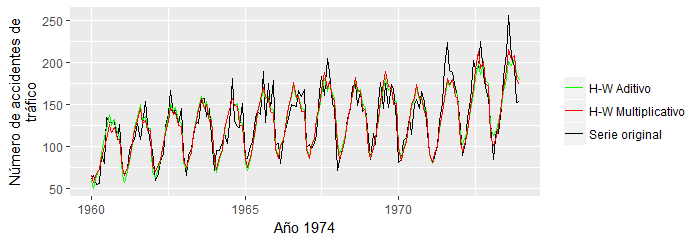
\includegraphics[scale = 0.7]{Images/Modelizacion/313.png}}
    \caption{Distintos ajustes de \PVerb{hw()}}
    \label{hw_fit}
\end{figure}

\begin{figure}
    \centering
    \centerline{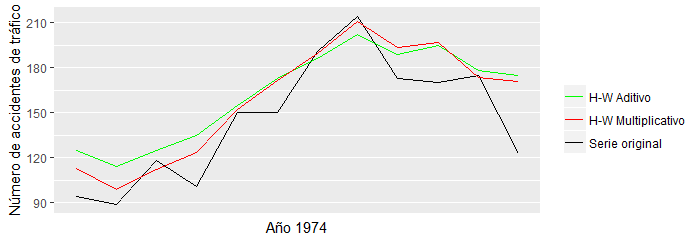
\includegraphics[scale = 0.7]{Images/Modelizacion/314.png}}
    \caption{Predicciones de los modelos correspondientes a \PVerb{hw()}}
    \label{hw_pred}
\end{figure}

\subsection{Red neuronal}
Son bien conocidas en el ámbito de la modelización las redes neuronales artificiales. Estos algoritmos consiguen adaptarse a una gran variedad de problemas debido a su característica estructura capaz de imitar el cerebro humano. Están estructuradas en capas formadas por unidades de procesamiento individual conocidas como neuronas. Estas están conectadas entre sí a través de conexiones ponderadas. La predicción realizada por la red dados unos \textit{inputs} determinados se obtiene en su capa final conocida como capa de salida. Estos algoritmos son realmente complejos, por ello nosotros nos centraremos únicamente en uno aplicado a series temporales univariantes.

En esta librería existe un método realmente útil encargado de implementar este tipo de redes neuronales conocido como $\verb!nnetar()!$.  Este método implementa una red \textit{feed-forward} con una única capa oculta o intermedia compuesta por $k$ neuronas. Toma como \textit{inputs} los últimos $p$ valores de la serie los cuales utiliza para realizar la predicción, estos valores obviamente van a estar rezagados respecto al que se busca predecir. Como este modelo también se apoya en modelos autorregresivos se conoce como \textit{Neural Network Auto Regressive  Model} y su notación es NNAR$(p, k)$.

Existe una pequeña variación de este modelo destinada a datos estacionales  que incluye además como \textit{inputs} los correspondientes valores en periodos anteriores de la observación a predecir, este modelo tiene la forma NNAR$(p, P, k)_M$ donde $M$ es la periodicidad de la serie y $P$ es el número de periodos anteriores de los que tomamos las observaciones como \textit{input}, es decir, en este caso tenemos una red con $k$ neuronas en su capa intermedia y con los siguientes \textit{inputs}:
\begin{equation}
    Y_{t-1}, Y_{t-2},...,Y_{t-p}, Y_{t-M}, Y_{t-2M},...,Y_{t-PM}
\end{equation}

Este método pertenece a la familia del método $\verb!nnet()!$ incluido en la librería $\verb!nnet!$ por lo que ambas comparten algunos argumentos. La sintaxis de $\verb!nnetar()!$ es la siguiente:
\begin{Verbatim}[fontsize=\footnotesize]
nnetar(y, p, P = 1, size, repeats = 20, decay, ...)
\end{Verbatim}

A través del argumento $\verb!y!$ se introduce la serie a modelizar y por $\verb!p!$ y $\verb!P!$ los parámetros ya comentados. El argumento $\verb!size!$ se corresponde con $k$, es decir, el número de neuronas que conforman la capa oculta. El entrenamiento de la red consiste en estimar los pesos que ponderan las conexiones entre neuronas, estos pesos se van actualizando a medida que le vamos pasando observaciones de la serie durante el entrenamiento por lo que es necesario iniciarles aleatoriamente. Para evitar la influencia de la aleatoriedad en los resultados se entrenan varias redes cada una con unos pesos iniciales distintos y se utiliza las media de las predicciones de todas ellas como predicción final. Este número de redes se introduce al modelo a través del argumento $\verb!repeats!$.

A continuación se ajusta una red neuronal con todos los argumentos por defecto y se predice el año 1974 de nuestra serie:
\begin{Verbatim}[fontsize=\footnotesize, numbers = left]
model <- nnetar(acc.train)
pred <- forecast(model, h = 12)
summary(model)
\end{Verbatim}

Observando los valores de los parámetros de nuestro modelo observamos que ha seleccionado $p = 1$, $P = 1$ y $k = 1$, por lo que parece que la estructura de nuestra red es bastante sencilla. El RMSE y el MAE en el conjunto de \textit{test} son 31.971323 y 26.22965 respectivamente, sin embargo en el conjunto de \textit{training} toman los valores 4.062094 y 3.12345. Esta diferencia es un indicador de que algo está fallando. En este tipo de modelos enmarcados dentro del \textit{machine learning} se suele dar con frecuencia un problema bastante común conocido como \textit{overfitting} causado por un sobreajuste del modelo en el conjunto de \textit{training} que hace que la inferencia sobre el conjunto de \textit{test} sea pésima. Para evitar esto se suele introducir un parámetro de regularización que limita al modelo obligándolo a suavizar su ajuste sobre el conjunto de \textit{training} para así poder obtener unas mejores inferencias. Este parámetro se introduce a partir del argumento $\verb!decay!$.

Para saber qué valor dar al parámetro de regularización  vamos a estudiar su comportamiento, para ello vamos a ejecutar varios modelos con valores de $\verb!decay!$ distintos y vamos a estudiar su MAE. En la Figura \ref{decay} se puede apreciar como el MAE desciende a medida que aumenta el parámetro de regularización, sin embargo cuando el parámetro toma valores cercanos a 9 comienza a estabilizarse, esto significa que el valor idóneo de este parámetro está entre 9 y 10. Si ajustamos una red con un decay de 9.5 obtenemos un RMSE y MAE en el conjunto de \textit{test} de 17.41186 y 14.86415 respectivamente, el mejor hasta el momento. Parece que hemos solucionado el \textit{overfitting} del modelo anterior ya que para el conjunto de \textit{training} obtenemos unos valores de 19.84883 y 15.51073.
\begin{figure}
    \centering
    \centerline{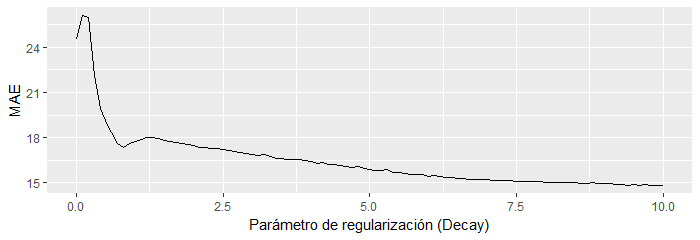
\includegraphics[scale = 0.7]{Images/Modelizacion/315.png}}
    \caption{Evolución del MAE respecto a \PVerb{decay}}
    \label{decay}
\end{figure}

Es posible mejorar el modelo introduciendo manualmente el resto de argumentos al método. Estudiando la evolución de los distintos parámetros de la misma forma (Anexo V) hemos llegado a la conclusión de que el modelo óptimo es el siguiente:
\begin{Verbatim}[fontsize=\footnotesize]
model <- nnetar(acc.train, repeats = 25, size = 20, decay = 9.5, p = 20, P = 4)
\end{Verbatim}

Obtenemos un MAE para el conjunto de test de 13.29118, el más bajo hasta el momento por lo que tiene sentido utilizar este modelo para predecir los accidentes de tráfico. En la Figura \ref{red} se muestra gráficamente el ajuste y se puede apreciar esa suavización de la predicción causada por el parámetro de regularización.
\begin{figure}
    \centering
    \centerline{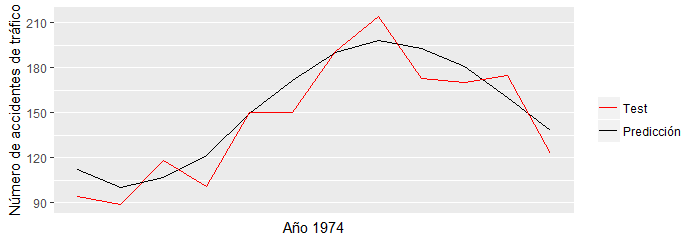
\includegraphics[scale = 0.7]{Images/Modelizacion/317.png}}
    \caption{Comparacións de la red óptima con el \textit{test}}
    \label{red}
\end{figure}

\subsection{Modelos ARIMA}
Los modelos ARIMA se utilizan con mucha frecuencia en la modelización de series temporales aunque, como ya se ha explicado, necesitan trabajar bajo unos supuestos más estrictos.

Uno de estos supuestos es el de homogeneidad de la varianza. Si la varianza de nuestra serie no se mantiene constante en el tiempo estaremos ante una serie no estacionaria y necesitaremos realizar algunas transformaciones a fin de poder aplicar esta clase de modelos. En la mayor parte de casos nos vale con aplicar logaritmos a nuestra serie, algo muy sencillo de hacer con $\verb!log()!$, sin embargo a veces esto no es suficiente y necesitaremos transformaciones más complejas como la de Box Cox. La librería $\verb!forecast!$ contiene un método muy bien optimizado para implementar esta transformación conocido como $\verb!BoxCox()!$. Su sintaxis es la siguiente:
\begin{Verbatim}[fontsize=\footnotesize]
BoxCox(x, lambda)
\end{Verbatim}

\noindent donde $\verb!x!$ recoge la serie a transformar y $\verb!lambda!$ el parámetro $\lambda$ que define la transformación. Este parámetro puede ser introducido manualmente por el usuario pero se suele utilizar el método $\verb!BoxCox.lambda()!$ que le selecciona automáticamente. Su sintaxis es la siguiente:
\begin{Verbatim}[fontsize=\footnotesize]
BoxCox.lambda(x, method = c("guerrero", "loglik"), lower = -1, upper = 2)
\end{Verbatim}

Recomiendo dejar todos los argumentos por defecto ya que así suele ofrecer muy buenos resultados. Para calcular nuestra serie transformada y mostrarla gráficamente bastaría con el siguiente código:
\begin{Verbatim}[fontsize=\footnotesize, numbers = left]
acc.train.trans <- BoxCox(x = acc.train, lambda = BoxCox.lambda(acc.train)
autoplot(acc.train.trans)
\end{Verbatim}

Apenas se aprecian diferencias entre las series transformadas y la original por lo que vamos a suponer que efectivamente nuestra serie es estacionaria en varianza.

Analizando visualmente la serie se puede apreciar que la tendencia no es constante sino que varía respecto al tiempo. Para cerciorarnos de esto vamos a aplicar el test de la raíz unitaria de Dickey-Fuller a través del método $\verb!ndiffs()!$. Obtenemos una salida de 1 lo que significa que es necesario diferenciar la serie una vez para sea estacionaria. Existe una variación de este método conocido como $\verb!nsdiffs()!$ orientado a comprobar si es necesario aplicar diferencias en la parte estacional del modelo, en este caso nos arroja una salida de 0 por lo que parece que no es necesario realizar ninguna diferencia a nivel estacional.

Una vez sabemos que nuestra serie es estacionaria podemos pasar a estudiar sus correspondientes correlogramas formados tanto a partir de la función de autocorrelación estándar como de la parcial. Los métodos encargados de implementar esto son $\verb!Acf()!$ y $\verb!Pacf()!$ respectivamente. Ambos comparten la misma sintaxis:
\begin{Verbatim}[fontsize=\footnotesize]
Acf(x, lag.max = NULL, ...)
\end{Verbatim}

A través de $\verb!x!$ introducimos la serie y con $\verb!lag.max!$ fijamos el número máximo de rezagos para los que calcular el correspondiente correlograma. En la Figura \ref{corr} se muestran estos correlogramas para nuestra serie diferenciada. El ACF parece mostrar correlaciones significativas para los rezagos 6, 12, 18 y 24.  Como estamos trabajando bajo un supuesto de estacionalidad anual vamos a fijar un $Q = 2$ y un $q = 0$ ya que parece no haber correlaciones significativas para la parte no estacional. El PACF no parece mostrar ninguna correlación significativa útil ni para la parte estacional ni para la no estacional por lo que vamos a fijar $p = 0$ y $P = 0$. Fijado esto el modelo a ajustar es un SARIMA$(0,1,0)(0,0,2)_{12}$ (en el Anexo VI se muestra una breve explicación de este tipo de modelos).
\begin{figure} [t]
\begin{subfigure}{.5\textwidth}
  \centering
  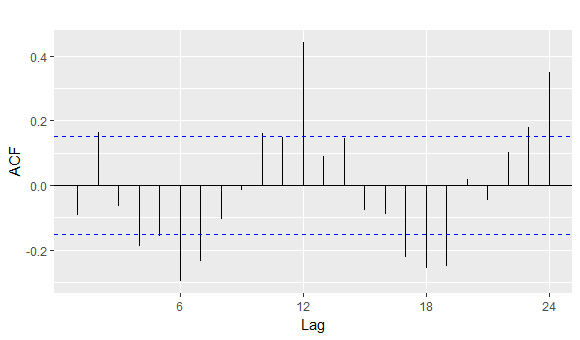
\includegraphics[width=.8\linewidth]{Images/Modelizacion/3181.png}
  \caption{ACF}
  \label{fig:sfig1}
\end{subfigure}
\begin{subfigure}{.5\textwidth}
  \centering
  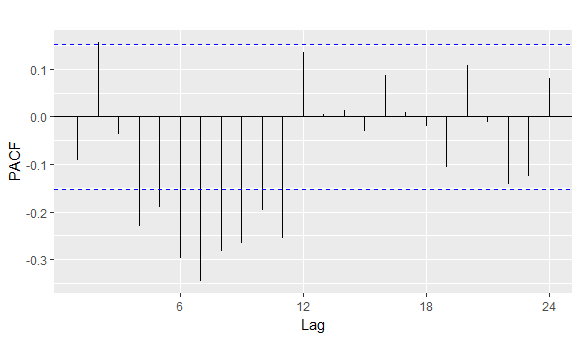
\includegraphics[width=.8\linewidth]{Images/Modelizacion/3182.png}
  \caption{PACF}
  \label{fig:sfig2}
\end{subfigure}
\caption{Correlogramas para la serie diferenciada de accidentes de tráfico en Ontario}
\label{corr}
\end{figure}

Para ajustar el modelo vamos a utilizar el método $\verb!Arima()!$ propio de esta librería y que se deriva del $\verb!arima()!$ de $\verb!stats()!$. Este método ofrece una personalización más completa del modelo además de una mejor integración con el entorno de la librería $\verb!forecast!$. Su sintaxis es la siguiente:
\begin{Verbatim}[fontsize=\footnotesize]
Arima(y, order = c(0,0,0), seasonal = c(0,0,0),
      include.mean = TRUE, include.drift = FALSE, …)
\end{Verbatim}

A través de $\verb!y!$ introducimos la serie y en $\verb!order!$ y $\verb!seasonal!$ introducimos los órdenes y las diferencias realizadas sobre cada una de las partes, respectivamente. Con el argumento $\verb!include.mean!$ se controla la inclusión del intercepto $c$ en el modelo. Si se fija como $\verb!TRUE!$ tenemos que $c \simeq \mu$ para $d = 0$ y $c = 0$ para $d > 0$. En caso de que se pase como $\verb!FALSE!$, $c = 0$ para cualquier $d$. El argumento $\verb!include.drift!$ permite también incorporar una variación de este intercepto al modelo cuando $d = 1$. El modelo generado por este método se trata de la misma forma que todos los anteriores. A continuación se muestra cómo generamos el modelo mencionado anteriormente y sus características principales:
\begin{Verbatim}[fontsize=\footnotesize, numbers = left]
model <- Arima(acc.train, order = c(0,1,0), seasonal = c(0,0,2))
summary(model)
\end{Verbatim}

La salida generada por este código es la siguiente:
\begin{Verbatim}[fontsize=\footnotesize]
          Series: acc.train
          ARIMA(0,1,0)(0,0,2)[12]

          Coefficients:
                  sma1    sma2
                0.3918  0.2472
          s.e.  0.0788  0.0739

          sigma^2 estimated as 605.1:  log likelihood=-772.19
          AIC=1550.38   AICc=1550.53   BIC=1559.73

          Training set error measures:
                              ME     RMSE      MAE       MPE
          Training set 0.3068305 24.37856 19.84998 -1.632044
                                     MAPE     MASE       ACF1
                                 15.91416 1.119117 -0.2672489
\end{Verbatim}

Con esta información tenemos que el modelo ajustado es:
\begin{equation}
    \Delta Y_t = 0.3918 \thinspace Y_{t-12} + 0.2472 \thinspace Y_{t-24} + a_t
\end{equation}

También nos ofrece unas medidas de ajuste conocidas como criterios de información. Nosotros nos centraremos en el de Akaike (AIC) ya que el resto son variaciones de este. Se calcula de la siguiente manera:
\begin{equation}
    AIC = -2 \thinspace \ln (L) + 2k
\end{equation}

\noindent donde $k$ es el número de parámetros que se han necesitado estimar y $L$ el máximo valor de la correspondiente función de verosimilitud. Estas medidas relativas son útiles ya que no solo comparan modelos de acuerdo a su ajuste sino que también penalizan por el número de parámetros estimados. En este caso tenemos que el AIC toma el valor de 1550.38. También nos muestra el MAE del conjunto de training que toma el valor de 19.84998.

Al igual que con los modelos anteriores vamos a realizar las predicciones para el año 1974 a través de $\verb!forecast()!$ y vamos a comparar a través de $\verb!accuracy()!$ los verdaderos valores ($\verb!acc.test!$) con los predichos por el modelo. Para el conjunto de test obtenemos un MAE de 22.19949 por lo que parece que no consigue igualar a algunos de los modelos ajustados anteriormente. Si estudiamos los residuos vemos que están correlacionados entre sí ya que obtenemos un p-valor para el test de Ljung Box de prácticamente cero. Esto significa que este modelo no es el óptimo ya que no consigue recoger toda la información presente en los datos.

Aunque ya hemos visto que no parecía ser necesario diferenciar la serie estacionalmente para lograr estacionariedad vamos a realizar esta diferenciación a fin de ver si el modelo que arroja ofrece mejores resultados que el anterior. Para ello vamos a aplicar a nuestra serie el método $\verb!diff()!$ con $\PVerb{lag} = 12$. En la Figura \ref{diff} se muestra la representación de la serie diferenciada junto a su correspondiente ACF y PACF.
\begin{figure}
\begin{subfigure}{.5\linewidth}
\centering
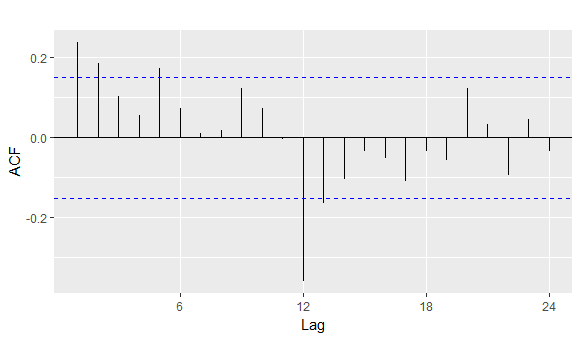
\includegraphics[width=.7\linewidth]{Images/Modelizacion/3192.png}
\caption{ACF}
\label{fig:sub1}
\end{subfigure}%
\begin{subfigure}{.5\linewidth}
\centering
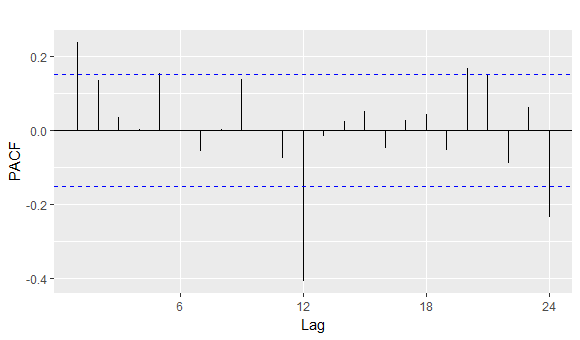
\includegraphics[width=.7\linewidth]{Images/Modelizacion/3193.png}
\caption{PACF}
\label{fig:sub2}
\end{subfigure}\\[1ex]
\begin{subfigure}{\linewidth}
\centering
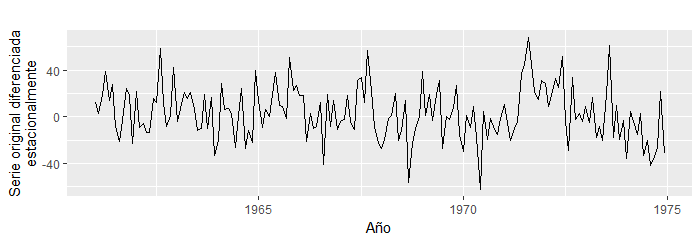
\includegraphics[width=.5\linewidth]{Images/Modelizacion/3191.png}
\caption{Serie diferenciada}
\label{fig:sub3}
\end{subfigure}
\caption{Estudio de la serie original diferenciada estacionalmente}
\label{diff}
\end{figure}

En el ACF apreciamos una correlación significativa en el primer rezago por lo que fijamos $q = 1$ y otra en el rezago 12 por lo que $Q = 1$. En el PACF ocurre lo mismo solo que en este caso también la correlación del rezago 24 parece significativa por lo que $p = 1$ y $P = 2$.

Vamos a ajustar dos modelos uno con el intercepto provisto por $\verb!include.driftt!$ y otro sin él. En la Tabla \ref{comp_1} se muestran las medidas de ajuste para ambos modelos.
\begin{table}[]
\centering
\label{my-label}
\begin{tabular}{|l|c|c|}
\hline
\multicolumn{1}{|c|}{} & \PVerb{include.drift = FALSE} & \PVerb{include.drift = TRUE} \\ \hline
AIC                    & 1367.68              & \textbf{1359.82}      \\ \hline
AICc                   & 1368.25              & \textbf{1360.58}      \\ \hline
BIC                    & 1385.98              & \textbf{1381.17}      \\ \hline
MAE en el test         & 19.22651             & \textbf{17.0999}      \\ \hline
P-valor (Ljung Box)    & 0.04321              & \textbf{0.2748}       \\ \hline
\end{tabular}
\caption{Comparación del ajuste de un SARIMA$(1,0,1)(2,1,1)_{12}$ con y sin intercepto}
\label{comp_1}
\end{table}

Se puede apreciar como el modelo con intercepto consigue mejores resultados en todos los aspectos. Tanto los criterios de información como el MAE son más bajos, además hemos conseguido que los residuos sean ruido blanco. No cabe duda de que en este caso el intercepto consigue mejorar notablemente el modelo. En la Figura \ref{comp_sarimas} se aprecia como las predicciones del modelo con $\verb!include.driftt = TRUE!$ consiguen ajustarse mejor a los valores reales gracias a la modificación en su nivel dada por la inclusión del intercepto.
\begin{figure}
    \centering
    \centerline{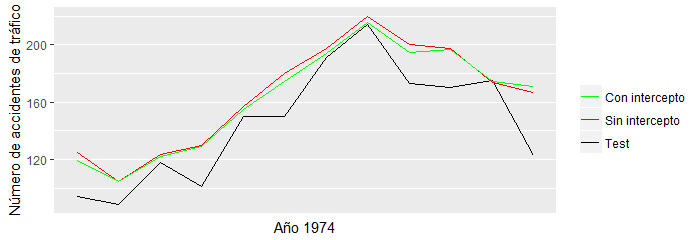
\includegraphics[scale = 0.7]{Images/Modelizacion/320.png}}
    \caption{Comparación de las predicciones del SARIMA$(1,0,1)(2,1,1)_{12}$ con y sin intercepto}
    \label{comp_sarimas}
\end{figure}

Existe un método realmente útil en esta librería encargado de seleccionar automáticamente el modelo, conocido como $\verb!auto.arima()!$. Se basa en un algoritmo que mediante la combinación del test de raíz unitaria, la optimización de los criterios de información y de la función de verosimilitud es capaz de seleccionar el modelo óptimo entre varios posibles. Los pasos que este algoritmo lleva a cabo son los siguientes:
\begin{enumerate*}
  \item Utiliza el test de la raíz unitaria de KPSS para determinar el número de diferencias necesarias, $d$, para lograr estacionariedad.
  \item A través del test OCSB de raíces unitarias estacionales determina el número necesario de diferencias $D$.
  \item Se selecciona $p$, $q$, $P$ y $Q$ de entre unos modelos iniciales de forma que se minimice el AICc, que no es más que una variación del AIC para muestras pequeñas.
  \item Se va variando progresivamente el orden y la presencia del intercepto del modelo seleccionado. Si el nuevo modelo tiene un AICc más bajo se toma este como referencia, en caso contrario se sigue con el anterior.
  \item Este último paso se repite hasta que no es posible encontrar otro modelo con un AICc más bajo.
  \item Ofrece como salida el último modelo seleccionado que, dado el funcionamiento del algoritmo, es el que minimiza el AICc.
\end{enumerate*}
\newpage
El proceso de selección se puede personalizar gracias a la sintaxis del método:
\begin{Verbatim}[fontsize=\footnotesize]
auto.arima(y, d = NA, D = NA, max.p = 5, max.q = 5, max.P = 2, max.Q = 2, max.d = 2,
           max.D = 1, ic = ("aicc", "aic", "bic"), test = c("kpss", "adf", "pp"),
           seasonal.test = c("ocsb", "ch"),...)
\end{Verbatim}

A través de $\verb!y!$ se introduce la serie a modelizar y en $\verb!d!$ y $\verb!D!$ se puede introducir las diferencias a realizar en cada parte de la serie, en caso de dejar estos argumentos por defecto lo decidirá el propio método gracias a varios test de raíz unitaria. A través de $\verb!max.d!$ y $\verb!max.D!$ se puede acotar superiormente las diferencias sobre las que buscar el modelo óptimo. Esto último también se puede aplicar a los parámetros a través de $\verb!max.p!$, $\verb!max.q!$, $\verb!max.P!$ y $\verb!max.Q!$. Se puede seleccionar el test a usar para seleccionar $d$ y $D$ gracias a los argumentos $\verb!test!$ y $\verb!seasonal.test!$. A través de $\verb!ic!$ podemos decidir sobre qué criterio se va a realizar la búsqueda del modelo óptimo.

Si aplicamos este método a nuestra serie $\verb!acc.train!$ especificando únicamente que utilice el test aumentado de la raíz unitaria de Dickey-Fuller para seleccionar $d$ obtenemos un SARIMA$(1,0,0)(1,0,0)_{12}$. Este modelo tiene un AIC de 1514.47, más alto que los dos anteriores y además hay correlaciones entre sus residuos. A pesar de esto el MAE del conjunto de test es de 14.86938, el mejor hasta ahora de todos los modelos  ARIMA ajustados.

El modelo que nos ofrece $\verb!auto.arima()!$ depende principalmente del algoritmo de búsqueda. Con ligeras variaciones en algunos de sus argumentos es posible obtener resultados completamente distintos. Por defecto esta búsqueda está configurada para tener un coste computacional bajo, sin embargo es posible forzar al algoritmo a que haga una búsqueda más exhaustiva pasando $\verb!stepwise!$ y $\verb!approximation!$ como $\verb!FALSE!$. Estos argumentos controlan el número de modelos sobre los que se realiza la búsqueda y la exactitud de los criterios usados. El argumento $\verb!max.order!$ fija el orden máximo del modelo de acuerdo a $p + q + P + Q$.

Hemos realizado esta búsqueda para nuestra serie fijando el $\verb!max.order!$ en 7. El modelo que nos ofrece es un SARIMA$(2,0,0)(2,0,0)_{12}$. En este caso el AIC es 1499.24 y el MAE de 14.96979. En el modelo anterior estamos realizando una buena predicción a pesar de tener un AIC superior al resto de modelos. En la Figura \ref{sarima_test} se aprecia como este modelo consigue detectar muy bien las fluctuaciones estacionales del conjunto de \textit{test}.
\begin{figure}
    \centering
    \centerline{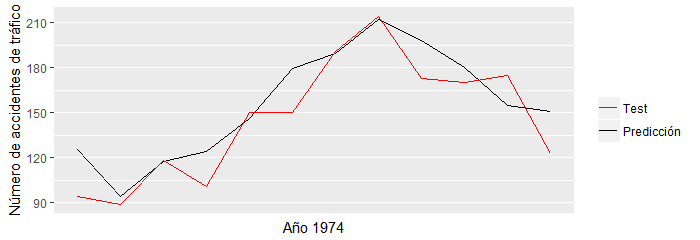
\includegraphics[scale = 0.7]{Images/Modelizacion/321.png}}
    \caption{Comparación de las predicciones del SARIMA$(2,0,0)(2,0,0)_{12}$ con el \textit{test}}
    \label{sarima_test}
\end{figure}

En la Tabla \ref{comp_2} se pueden ver las medidas de ajuste de distintos modelos. Se puede apreciar como el modelo con los mejores criterios de información es el SARIMA$(1,0,1)(2,1,1)_{12}$ con intercepto, además de que es el único con unos residuos puramente aleatorios. Sin embargo no es el que mejor predice ya que el mejor MAE le posee el SARIMA$(1,0,0)(1,0,0)_{12}$. Realmente no podemos decir que hay un modelo que destaque sobre los demás sino que algunos son mejores que otros en ciertos aspectos. Si queremos dar preponderancia al ajuste deberíamos fijarnos más en los criterios de información y en la aleatoriedad de los residuos mientras que si lo que buscamos son predicciones a corto-medio plazo deberíamos tener en cuenta medidas como el MAE. Al fin y al cabo la elección del modelo óptimo queda al criterio del usuario.
\begin{table}[]
\centering
\label{my-label}
\begin{tabular}{|l|c|c|c|c|c|}
\hline
\multicolumn{1}{|c|}{}                & AIC              & AICc             & BIC & MAE & Ljung Box \\ \hline
$(0,1,0)(0,0,2)_{12}$               & 1550.38          & 1550.53          & 1559.73                  & 22.19949                 & $\sim 0$                                   \\ \hline
$(1,0,1)(2,1,1)_{12 \thinspace sin \thinspace int}$ & 1367.68          & 1368.25          & 1385.98                  & 19.22651                 & 0.04321                                  \\ \hline
$(1,0,1)(2,1,1)_{12 \thinspace con \thinspace int}$ & \textbf{1359.82} & \textbf{1360.58} & \textbf{1381.17}         & 17.09992                 & \textbf{0.2748}                          \\ \hline
$(1,0,0)(1,0,0)_{12}$               & 1514.22          & 1514.47          & 1526.72                  & \textbf{14.86938}        & 0.00085                                   \\ \hline
$(2,0,0)(2,0,0)_{12}$                & 1499.24          & 1499.77          & 1517.99                  & \textbf{14.96979}        & 0.002708                                  \\ \hline
$(1,1,4)(2,0,0)_{12}$               & 1485.29          & 1486.2           & 1510.24                  & 23.44705                 & 0.01353                                  \\ \hline
\end{tabular}
\caption{Comparación de los distintos SARIMA ajustados}
\label{comp_2}
\end{table}

\section{TSeries Package}
La librería $\verb!tseries!$ contiene métodos tanto de preprocesado como de modelización de serie temporales, además de varios test estadísticos orientados a series temporales. Aunque muchos de sus métodos están orientados al análisis de series financieras es posible aplicarlos, tras las transformaciones oportunas, a series con una temática más general \cite{tseries}.

Vamos a cargar los datos en el formato $\verb!zoo!$ y $\verb!ts!$ aunque básicamente utilizaremos este último dado que nos apoyaremos en algunos métodos de las librerías $\verb!stats!$ y $\verb!forecast!$ (se puede ver el código en el Anexo VII).

\subsection{Preprocesado}
Comenzaremos desestacionalizando nuestra serie a fin de poder aplicar más adelante un modelo ARMA. Para ello vamos a estimar las distintas componentes a través del método $\verb!decompose()!$ y con $\verb!seasadj()!$ de $\verb!forecast!$ vamos a eliminar la componente estacional. En esta ocasión vamos a trabajar bajo el supuesto de aditividad y además vamos a realizar la división en \textit{training} y \textit{test} después de la desestacionalización y no antes. El resultado se muestra en la Figura \ref{acc_deses}.
\begin{figure}
    \centering
    \centerline{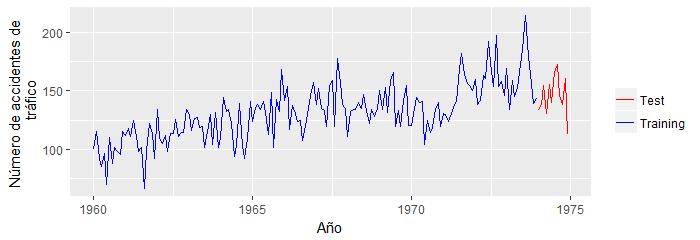
\includegraphics[scale = 0.7]{Images/Modelizacion/322.png}}
    \caption{Serie \PVerb{accidentes} desestacionalizada con \PVerb{seasadj()}}
    \label{acc_deses}
\end{figure}

Debido a la naturaleza del modelo a aplicar debemos trabajar bajo el supuesto de estacionariedad. Para ello aplicaremos tres test distintos implementados en esta librería:
\begin{itemize*}
  \item[$\bullet$] \textbf{Test aumentado de Dickey-Fuller}: Implementado por $\verb!adf.test()!$, nos permite contrastar tanto el supuesto de estacionariedad (raíz unitaria) como de explosividad (raíz fuera del círculo unidad). Para elegir entre un ajuste u otro debemos modificar el argumento $\verb!alternative!$ ($\verb!"stationary"!$ o $\verb!"explosive"!$).
  \item[$\bullet$] \textbf{Test de Philipps-Perron}: El método que lo implementa es $\verb!pp.test()!$ y funciona de la misma manera que $\verb!adf.test()!$. Este test se deriva del de Dickey-Fuller solo que utiliza técnicas no paramétricas para aproximar la distribución del estadístico.
  \item[$\bullet$] \textbf{Test de KPSS}: Contrasta la hipótesis nula de que la serie es estacionaria en tendencia frente a la presencia de raíz unitaria. Se implementa a través de $\verb!kpss.test()!$. Para trabajar bajo la tendencia aquí tratada se debe introducir el argumento $\verb!null!$ como $\verb!"Trend"!$.
\end{itemize*}

En los test de Dickey-Fuller y Phillipps-Perron estamos obteniendo unos p-valores para los contrastes de estacionariedad y explosividad de 0.01 y 0.99, respectivamente.  Esto significa que parece haber indicios de estacionariedad en nuestra serie ya que hemos rechazado la hipótesis nula de raíz unitaria y no hemos podido rechazar la de no explosividad. El p-valor para el test de KPSS es de 0.05506 por lo que no podemos rechazar la hipótesis nula de estacionariedad en tendencia, sin embargo si observamos la serie apreciamos que sí que parece haber tendencia no constante por lo que vamos a diferenciar la serie para eliminarla. El resultado se muestra en la Figura \ref{acc_deses_diff}.
\begin{figure}
    \centering
    \centerline{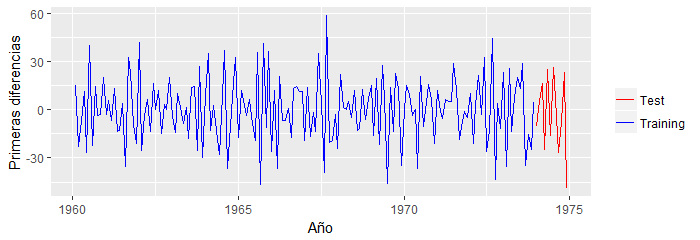
\includegraphics[scale = 0.7]{Images/Modelizacion/323.png}}
    \caption{Serie \PVerb{accidentes} desestacionalizada y diferenciada}
    \label{acc_deses_diff}
\end{figure}

Tras esta transformación obtenemos los mismos resultados en los test de Dickey-Fuller y Phillips-Perron, sin embargo ahora nos sale un p-valor para el test de KPSS de 0.1, lo que significa que no podemos rechazar la hipótesis de estacionariedad en tendencia. Trabajaremos con esta serie ya que parece haber fuertes evidencias estadísticas de estacionariedad.

Existen test encargados de contrastar la linealidad de la tendencia de series temporales a través de métodos basados en redes neuronales. Esta librería incorpora dos métodos capaces de implementar los test de no linealidad: Terasvirta y White. Aunque ambos tests funcionan de forma similar, el de White es más restrictivo ya que consigue diferenciar en el contraste la no linealidad arbitraria. Los respectivos métodos son $\verb!terasvirta.test()!$ y $\verb!white.test()!$ y trabajan bajo la hipótesis nula de linealidad en media. Para el tipo de serie que manejamos basta con dejar los argumentos por defecto. Obtenemos un p-valor de 0.8989 en el test de Terasvirta y de 0.7783 en el de White, por lo que nuestra serie parece seguir una tendencia lineal (algo lógico ya que hemos dejado la tendencia constante al diferenciar).

Existe un método en esta librería conocido como $\verb!maxdrawdown()!$ que se encarga de extraer la mayor disminución de la serie, es decir, nos devuelve el periodo con mayor diferencia entre el valor inicial y el final. En nuestro caso ese periodo se corresponde al comprendido entre septiembre de 1967 y julio de 1969, con una diferencia de 104.3482 unidades. Estas unidades ya no se pueden interpretar como accidentes ya que hemos realizado varias transformaciones a la serie.

\subsection{Técnicas de remuestreo}
Gracias al desarrollo de la computación se han popularizado las técnicas de remuestreo, una de las más conocidas es el \textit{bootstrap} \cite{efron_bootstrap_1979}. En ocasiones queremos estimar un parámetro poblacional y para ello contamos únicamente con una muestra. Con esta técnica extraemos submuestras de esa muestra a través de un muestreo aleatorio con reposición y de estas submuestras se obtiene el estadístico deseado. Esto se repite un gran número de veces pudiendo así construir una aproximación de la distribución del estadístico a través de las submuestras.

Esta técnica se puede aplicar a series temporales, solo que necesitamos hacer algunas modificaciones. No podemos aplicar un muestreo aleatorio ya que perderíamos la característica que define a las series temporales, la correlación temporal. En este caso se utiliza una variación del \textit{bootstrap} original conocido como \textit{bootstrap} por bloques. El método encargado de implementar esto es $\verb!tsbootstrap()!$ y su sintaxis es la siguiente:
\begin{Verbatim}[fontsize=\footnotesize]
tsbootstrap(x, nb = 1, statistic = NULL, m = 1, b = NULL,
            type = c("stationary","block"), ...)
\end{Verbatim}

A través de $\verb!x!$ se introduce la serie y a partir de $\verb!nb!$ el número de series a generar (submuestras). El argumento $\verb!type!$ define el tipo de \textit{bootstrap} a aplicar, las opciones disponibles son las siguientes:
\begin{itemize*}
  \item[$\bullet$] \textbf{Por bloques} (\PVerb{"block"}): La serie se divide en  $n-b+1$ bloques de longitud $b$ de forma que el primer bloque contendrá las observaciones $Y_1,...,Y_b$, el segundo las observaciones $Y_2,...,Y_{b+1}$, etc… Sobre estos bloques se hace un muestreo aleatorio con remplazamiento seleccionando $n/b$ bloques y se combinan sin alterar su orden en la serie original de forma que obtenemos una nueva serie capaz de replicar la autocorrelación temporal.
  \item[$\bullet$] \textbf{Estacionario} (\PVerb{"stationary"}): El procedimiento es el mismo solo que en este caso $b$ no es fijo sino que varía aleatoriamente. Con esta pequeña modificación nos aseguramos la estacionariedad de la nueva serie.
\end{itemize*}

El argumento $\verb!b!$ fija la longitud de los bloques si trabajamos bajo el tipo $\verb!"block"!$, en caso de hacerlo bajo $\verb!"stationary"!$ fija la media de la longitud de los bloques, es decir, la media de los valores aleatorios generados. Se recomienda que $b$ aumente con $n$, por ello por defecto el valor de $b$ es proporcional a $n^3$. Si el argumento $\verb!statistic!$ se deja por defecto el método nos devolverá la serie remuestrada, en caso de que se introduzca alguna función como $\verb!mean()!$ o $\verb!sd()!$, nos devolverá el estadístico aplicado a la serie original y la estimación del sesgo y del error estándar a través de las series generadas por el \textit{bootstrap}.

El argumento $\verb!m!$ introduce una pequeña variación en el \textit{bootstrap}. Por defecto vale 1, esto mantiene el proceso como se ha descrito pero si $\PVerb{m} > 1$ divide la serie original en bloques de longitud $m$ y aplica el \textit{bootstrap} individualmente a esos bloques, en vez de a la serie en su totalidad. Como en este caso la serie original se ha divido, el estadístico aplicado a la serie original varía. En la Figura \ref{bootstrap} se muestran las series generadas por un \textit{bootstrap} por bloques y estacionario con los argumentos $\verb!m!$ y $\verb!b!$ por defecto.

\begin{figure}
    \centering
    \centerline{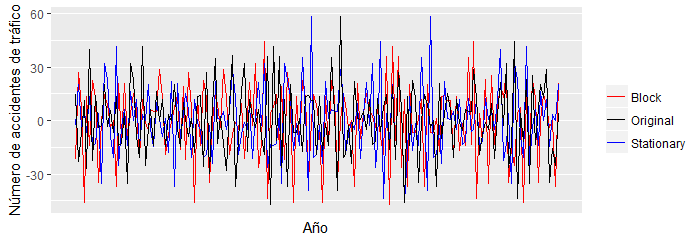
\includegraphics[scale = 0.7]{Images/Modelizacion/32413242.png}}
    \caption{El método \PVerb{tsbootstrap()} aplicado a la serie \PVerb{acc.train.dif.adj}}
    \label{bootstrap}
\end{figure}

Vamos a definir una función $\verb!initial.acf()!$ que nos devuelva los siete primeros valores del correlograma de la función de autocorrelación (excluyendo el primero). Tras esto vamos a hacer un \textit{bootstrap} estacionario sobre nuestra serie para intentar estimar estas correlaciones a través de 500 submuestras de la serie. La salida resultante es la siguiente:
\vspace{1cm}
\begin{Verbatim}[fontsize=\footnotesize]
          Call:
          tsbootstrap(x = acc.train.dif.adj, nb = 500, statistic =
          initial.acf, type = "stationary")

          Resampled Statistic(s):
             original      bias std. error
          t1 -0.46105  0.032406    0.04939
          t2  0.05999 -0.021088    0.08265
          t3 -0.00991  0.010304    0.08036
          t4 -0.11464  0.016317    0.08634
          t5  0.07060  0.001765    0.08768
          t6 -0.01765  0.009458    0.07539
          t7 -0.08207  0.011581    0.07784
\end{Verbatim}

En primer lugar nos muestra las características del \textit{bootstrap} utilizado. Después vemos los valores de los estadísticos (en este caso las autocorrelaciones) en la muestra acompañados del sesgo y el error estándar obtenidos gracias al \textit{bootstrap}.

Un método similar incluido en esta librería es $\verb!surrogate()!$. Las series temporales no son más que funciones periódicas en el tiempo por lo que en ocasiones se utilizan transformadas de Fourier para describirlas. Este método recurre a este tipo de técnicas para generar subseries con una estructura similar a la original. Su sintaxis es la siguiente:
\begin{Verbatim}[fontsize=\footnotesize]
surrogate(x, ns = 1, fft = FALSE, amplitude = FALSE, statistic = NULL, ...)
\end{Verbatim}

A través de $\verb!x!$ se introduce la serie y en $\verb!ns!$ se indica el número de series a generar. Si los argumentos $\verb!fft!$ y $\verb!amplitude!$ se dejan en $\verb!FALSE!$ lo único que hace es generar las nuevas series a partir de permutaciones de la original perdiendo así toda la correlación temporal. En este tipo de técnicas el espectro recoge la distribución de amplitudes que definen al proceso modelado, el argumento $\verb!fft!$ consigue generar una nueva serie basada en el espectro de la original introduciendo cierta aleatorización en la fase de los coeficientes de Fourier. El argumento $\verb!amplitude!$ consigue mantener en las nuevas series las amplitudes de la original. En la Figura \ref{surrogate} se muestra la serie original junto a una generada a partir de este método con los argumentos $\verb!fft!$ y $\verb!amplitude!$ como $\verb!TRUE!$.
\begin{figure}
    \centering
    \centerline{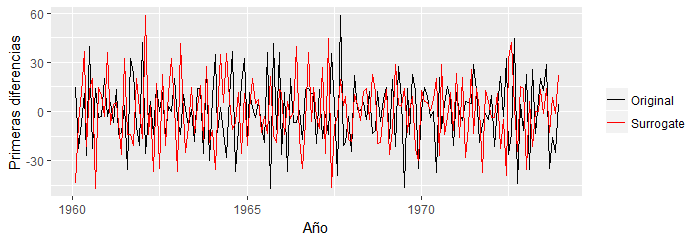
\includegraphics[scale = 0.7]{Images/Modelizacion/325.png}}
    \caption{El método \PVerb{surrogate()} aplicado a la serie \PVerb{acc.train.dif.adj}}
    \label{surrogate}
\end{figure}

\subsection{Modelos ARMA}
Una vez preparada la serie vamos a ajustarle un modelo ARMA. Como esta librería no incluye ningún método para la detección automática del orden de los parámetros vamos a estudiar sus correlogramas a partir de los métodos $\verb!Acf()!$ y $\verb!Pacf()!$ de la librería $\verb!forecast!$. Los resultados se muestran en la Figura \ref{a_p}. En el ACF se puede apreciar como únicamente la primera autocorrelación es significativa por lo que vamos a suponer $q = 1$ para la parte de medias móviles. En el PACF vemos que tanto la primera como la segunda autocorrelación son significativas, considerando parsimoniosidad vamos a suponer $p = 1$ para la parte autorregresiva.
\begin{figure} [t]
\begin{subfigure}{.5\textwidth}
  \centering
  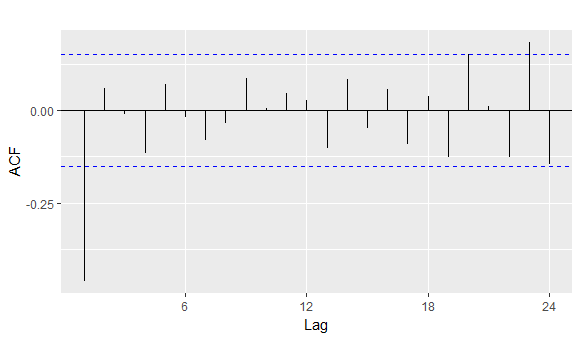
\includegraphics[width=.8\linewidth]{Images/Modelizacion/3261.png}
  \caption{ACF}
  \label{fig:sfig1}
\end{subfigure}
\begin{subfigure}{.5\textwidth}
  \centering
  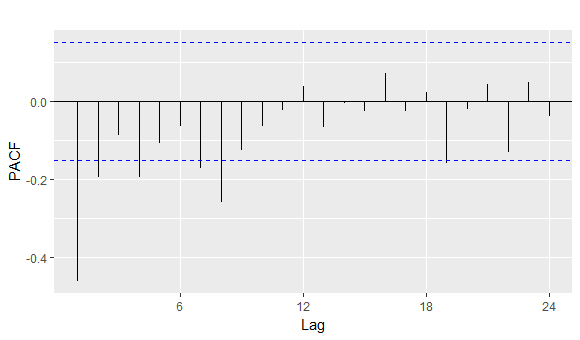
\includegraphics[width=.8\linewidth]{Images/Modelizacion/3262.png}
  \caption{PACF}
  \label{fig:sfig2}
\end{subfigure}
\caption{Correlogramas para la serie \PVerb{acc.train.dif.adj}}
\label{a_p}
\end{figure}

El método encargado de implementar los modelos ARMA en esta librería es $\verb!arma()!$. Su sintaxis es similar al $\verb!Arima()!$ de $\verb!forecast!$ ya que ambos se sustentan en el $\verb!arima()!$ de $\verb!stats!$:
\begin{Verbatim}[fontsize=\footnotesize]
arma(x, order = c(1, 1), lag = NULL, coef = NULL,
     include.intercept = TRUE, qr.tol = 1e-07, ...)
\end{Verbatim}

En $\verb!x!$ se introduce la serie a modelizar y tanto en $\verb!order!$ como en $\verb!lag!$ se puede introducir los órdenes de la parte autorregresiva y de la medias móviles. Si se introduce ambos argumentos se da prioridad a lo especificado en $\verb!order!$. A través del argumento $\verb!coef!$ se puede introducir una inicialización personalizada de los coeficientes para el proceso de estimación, recomiendo dejarlo por defecto. Con $\verb!include.intercept!$ incluimos el intercepto en el modelo y con $\verb!qr.tol!$ definimos la tolerancia que se utiliza para calcular el error estándar de los coeficientes. Para ajustar un ARMA$(1,1)$ sin intercepto a nuestra serie debemos escribir el siguiente código:
\begin{Verbatim}[fontsize=\footnotesize, numbers = left]
model.1 <- arma(acc.train.dif.adj, order = c(1,1), include.intercept = FALSE)
summary(model)
\end{Verbatim}

Al trabajar bajo la serie original diferenciada lo que realmente estamos ajustando es un ARIMA$(1,1,1)$. Estamos obteniendo un AIC de 1419.3 que aunque no es el mejor supera al de otros modelos ajustados con $\verb!forecast!$. Si graficamos el correlograma de los residuos vemos que ninguna autocorrelación es significativa por lo que parece que el modelo recoge todos los patrones de la serie. A través del método $\verb!jarque.bera.test()!$ incluido en este librería vamos a contrastar la normalidad de los residuos con el test de Jarque Bera. Obtenemos un p-valor de 0.5357 por lo que podemos afirmar que los residuos siguen una distribución normal, confirmando lo visto en el correlograma.  Otro método bastante útil para estudiar los residuos es $\verb!bds.test()!$. Este método implementa el test no paramétrico de BDS que contrasta la hipótesis nula de que los datos son independientes e idénticamente distribuidos (i.i.d). Su sintaxis es la siguiente:
\begin{Verbatim}[fontsize=\footnotesize, numbers = left]
bds.test(x, m = 3, eps = seq(0.5 * sd(x), 2 * sd(x),
                             length = 4),...)
\end{Verbatim}

Para ver cómo funciona este test definamos las siguientes probabilidades:
\begin{equation}
    P_1 = P(\lvert Y_i - Y_j \lvert < \epsilon)\quad \text{con} \quad i \neq j, \quad i,j \in T
\end{equation}
\begin{equation}
    P_m = P(\lvert Y_i - Y_j \lvert < \epsilon, \lvert Y_{i-1} - Y_{j-1} \lvert < \epsilon,...,\lvert Y_{i-m} - Y_{j-m} \lvert < \epsilon)
\end{equation}

Lo que estamos calculando en (68) es la probabilidad de que dos observaciones de nuestra serie no disten más de $\epsilon$, sin embargo en (69) estamos calculando la probabilidad de que tanto esas dos observaciones como sus $m$ anteriores no disten entre sí más de $\epsilon$. Si la serie $Y_t$ es independiente e idénticamente distribuida (i.i.d) por definición se tiene que:
\begin{equation}
    {P_1}^m = P_m
\end{equation}

Por lo tanto el test BSD contrasta lo siguiente:
\begin{align}
    H_0 &: {P_1}^m = P_m \rightarrow i.i.d\\
    H_1 &: {P_1}^m \neq P_m \rightarrow no \: i.i.d
\end{align}

El argumento $\verb!m!$ fija hasta dónde llega $m$ partiendo de 2 (por defecto es 3 por lo que $\verb!m!$ tomará los valores 2 y 3) y $\verb!eps!$ los valores de $\epsilon$. Como salida obtendremos $m \times \epsilon$ p-valores correspondientes a los resultados del test para las distintas combinaciones. Los p-valores para nuestros residuos dejando los argumentos por defecto son los siguientes:
\begin{Verbatim}[fontsize=\footnotesize]
         p-value =
               [ 8.3335 ] [ 16.667 ] [ 25.0004 ] [ 33.3339 ]
         [ 2 ]     0.4068     0.4443      0.4235      0.2465
         [ 3 ]     0.4032     0.9104      0.6961      0.4041
\end{Verbatim}

Obtenemos para todas las combinaciones p-valores mayores de 0.05 por lo que podemos afirmar que los residuos son i.i.d.

Hemos ajustado también un ARIMA$(2,1,1)$ para ver si mejora el modelo anterior (hemos tenido en cuenta la segunda autocorrelación de la Figura \ref{a_p}). Obtenemos un AIC de 1414.81, algo más bajo que el anterior. El test de Jarque Bera nos arroja un p-valor de 0.7782 y todos los p-valores del test BSD son mayores a 0.05. Todos estos indicios nos sugieren que este modelo también parece recoger todos los patrones contenidos en los datos ya que los residuos parecen ser ruido. En la Figura \ref{fit_arma} se muestra el ajuste de este último modelo.
\begin{figure}
    \centering
    \centerline{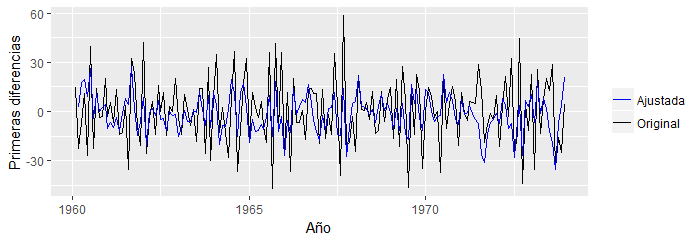
\includegraphics[scale = 0.7]{Images/Modelizacion/3272.png}}
    \caption{Ajuste del modelo ARIMA$(2,1,1)$ implementado con \PVerb{arma()}}
    \label{fit_arma}
\end{figure}

Esta librería no incluye ningún método para predecir a partir de los objetos generados por $\verb!arma()!$ por lo que no nos ha sido posible comparar ambos modelos de acuerdo a su poder predictivo.

\section{FitARMA Package}
Hasta ahora hemos visto librerías que incluían métodos generales para el análisis de series temporales, sin embargo existen otras más especializadas en ciertos aspectos de estas. La librería $\verb!FitARMA!$ únicamente incluye métodos orientados a la implementación de modelos ARIMA \cite{fitarma}.

Al no incluir modelos capaces de tratar la componente estacional vamos a desestacionalizar la serie de la misma manera en que lo hemos hecho para $\verb!tseries!$. Como la tendencia sigue dependiendo del tiempo también la vamos a diferenciar. El resultado son las series $\verb!acc.train.dif.adj!$ y $\verb!acc.test.dif.adj!$ que se mostraron en la Figura \ref{acc_deses_diff} (el código se encuentra en el Anexo VIII).

El método principal de esta librería es $\verb!FitARMA()!$ encargado de implementar los modelos ARIMA. Se caracteriza por el algoritmo de estimación que utiliza para ajustar el modelo a nuestros datos. Este algoritmo se sustenta en la estimación por máxima verosimilitud solo que consigue reducir los cálculos necesarios a través de una aproximación de esta \cite{fitarma-algoritmo}.

La sintaxis de este método es la siguiente:
\begin{Verbatim}[fontsize=\footnotesize]
FitARMA(z, order = c(0, 0, 0), demean = TRUE, MeanMLEQ = FALSE,
        pApprox = 30, MaxLag = 30)
\end{Verbatim}

A través de $\verb!z!$ introducimos la serie a modelizar y en $\verb!order!$ los valores de los parámetros $p$, $d$ y $q$ del modelo a ajustar. Si mantenemos $\verb!demean!$ como $\verb!TRUE!$ incluiremos el intercepto en el modelo. Si además queremos estimar el intercepto a través de este algoritmo debemos pasar el argumento $\verb!MeanMLEQ!$ como $\verb!TRUE!$. El algoritmo consigue aproximar la función de máximo verosimilitud del ARMA a través de un AR de un orden bastante superior, el argumento $\verb!pApprox!$ es el que indica al algoritmo el orden de este AR. Como este método implementa internamente el test de Ljung-Box deberemos indicarle a través de $\verb!MaxLag!$ el número de rezagos que debe utilizar.

Comenzaremos ajustando un ARMA$(2,1)$ a la serie $\verb!acc.train.dif.adj!$ dejando el resto de los argumentos del método por defecto. Si hacemos $\verb!summary()!$ sobre el modelo obtenemos la siguiente salida:
\begin{Verbatim}[fontsize=\footnotesize]
ARIMA(2,0,1)
length of series = 167 ,  number of parameters = 4
loglikelihood = -465.75 ,  aic = 939.5 ,  bic =  952
\end{Verbatim}

Destacar el bajo valor del AIC en comparación con los modelos ajustados con otras librerías. En este caso el AIC solo es comparable entre modelos con $d = 0$, además de entre aquellos ajustados con este método. Con $\verb!coef()!$ podemos obtener información acerca de los coeficientes del modelo, la correspondiente salida se muestra a continuación:
\begin{Verbatim}[fontsize=\footnotesize]
                        MLE         sd   Z-ratio
          phi(1)   0.2259977 0.08360269  2.703235
          phi(2)   0.1443701 0.08246120  1.750764
          theta(1) 0.9477932 0.02999630 31.597007
          mu       0.2586612 7.97254543  0.032444
\end{Verbatim}

Nos muestra tanto el valor de los coeficientes como sus desviaciones estándar. Además nos muestra también el estadístico $Z$ para cada uno de los coeficientes. Estamos trabajando a un nivel de significación de 0.05 que le corresponde un valor crítico de 1.96 por lo que únicamente $\phi_1$ y $\theta_1$ son significativamente distintos de cero.

Aunque es posible obtener las autocorrelaciones de los residuos a través del \textit{subsetting} $\verb!$racf!$ vamos a seguir recurriendo al método $\verb!Acf()!$. En la Figura \ref{residuos} se puede apreciar como ninguna autocorrelación resulta significativa. Además el test de Ljung-Box implementado por el propio método nos ofrece p-valores superiores a 0.05 para todos los rezagos.
\begin{figure}
    \centering
    \centerline{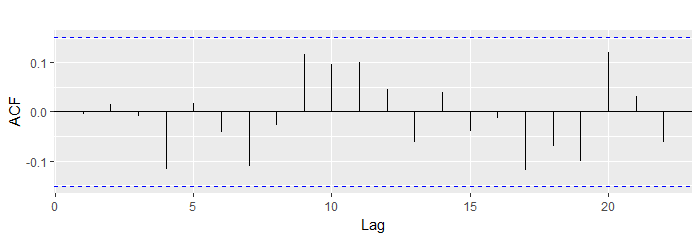
\includegraphics[scale = 0.7]{Images/Modelizacion/328.png}}
    \caption{Correlograma para los residuos del ARMA$(2,1)$}
    \label{residuos}
\end{figure}

El modelo anterior ha trabajado con $\PVerb{MeanMLEQ} = \PVerb{FALSE}$, vamos a pasarlo como $\verb!TRUE!$ para ver si afecta notablemente al ajuste. A continuación se muestra el código:
\begin{Verbatim}[fontsize=\footnotesize, numbers = left]
model.2 <- FitARMA(acc.train.dif.adj, order = c(2,0,1), MeanMLEQ = TRUE)
summary(model.2)
\end{Verbatim}

En este caso nos está devolviendo un AIC de 938.5 que es ligeramente menor al del modelo anterior, sin embargo la significatividad de los parámetros sigue siendo la misma. Los residuos de los modelos siguen mostrando suficientes evidencias estadísticas como para poder afirmar que son ruido. Aunque la diferencia en los AIC de los modelos es mínima supone una razón suficiente para hacernos decantar por este segundo modelo, es decir, por la estimación del intercepto a través del algoritmo de la librería. En la Figura \ref{arma_fitarma} se muestra el ajuste de este modelo a los datos.
\begin{figure}
    \centering
    \centerline{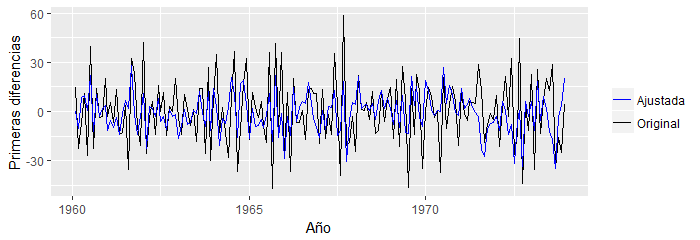
\includegraphics[scale = 0.7]{Images/Modelizacion/329.png}}
    \caption{Ajuste del modelo ARMA$(2,1)$ implementado con \PVerb{FitARMA()}}
    \label{arma_fitarma}
\end{figure}

Para intentar mejorar aún más este modelo vamos a intentar obtener el valor óptimo de $\verb!pApprox!$. Realizaremos ajustes para distintos valores de este parámetro y estudiaremos la verosimilitud para intentar localizar el óptimo. Probaremos a ajustar los distintos modelos de acuerdo a los valores 10, 20, 30, 40, 50, 60, 70 y 80 para $\verb!pApprox!$. En la Figura \ref{logaritmo} se muestra este estudio. Se puede observar que la verosimilitud desciende hasta alcanzar su valor mínimo con $\PVerb{pApprox} = 20$, sin embargo después parece incrementar a medida que se aumenta el valor del argumento. Lo que este estudio parece decirnos es que los valores de $\verb!pApprox!$ que maximizan la verosimilitud son aquellos más altos. Sabiendo esto vamos a ajustar el mismo modelo que antes solo que ahora vamos a pasar $\verb!pApprox!$ como 80, su $\verb!summary()!$ se muestra a continuación:
\begin{Verbatim}[fontsize=\footnotesize]
ARIMA(2,0,1)  With mean MLE.
length of series = 167 ,  number of parameters = 4
loglikelihood = -464.52 ,  aic = 937 ,  bic =  949.5
\end{Verbatim}

\begin{figure}
    \centering
    \centerline{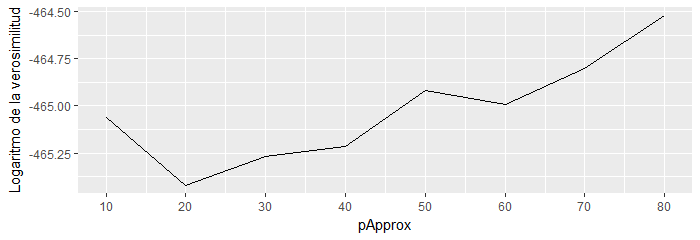
\includegraphics[scale = 0.7]{Images/Modelizacion/330.png}}
    \caption{Evolución del logaritmo de la verosimilitud respecto a \PVerb{pApprox}}
    \label{logaritmo}
\end{figure}

En este caso estamos obteniendo un AIC de 937, el más bajo hasta el momento. Este resultado parece mostrar que el argumento $\verb!pApprox!$ juega internamente un papel importante en el método.

A continuación vamos a comparar la eficiencia de este método respecto a sus equivalentes en las librerías $\verb!forecast!$ y $\verb!tseries!$ ($\verb!Arima()!$ y $\verb!arma()!$). Para ello vamos a estudiar sus tiempos con el método $\verb!system.time()!$. Ajustaremos a la serie $\verb!acc.train.dif.adj!$ un modelo ARMA$(2,1)$ a través de los tres métodos distintos y guardaremos el tiempo interno que tarda el ordenador en realizar cada uno de estos ajustes. Repetiremos este proceso 50 veces para poder apreciar cómo se comportan cada uno de los tres métodos.

En la Figura \ref{tiempos_modelos} se muestran los resultados de esta simulación. En el eje de las abscisas se muestra el número de simulación mientras que en el de las ordenadas el tiempo empleado por el ordenador para llevar a cabo el ajuste. Lo que más llama la atención es la gran diferencia de tiempos entre el método de $\verb!FitARMA!$ y los de $\verb!forecast!$ y $\verb!tseries!$. El algoritmo implementado en $\verb!FitARMA!$ ofrece rapidez para cantidades grandes de datos, sin embargo parece que para cantidades pequeñas se estanca, tardando casi tres veces más que el resto de métodos. Además parece mostrar un comportamiento muy errático, mostrando grandes variaciones en los tiempos cuando realmente su comportamiento debería mantenerse más o menos constante (la presencia de estas variaciones se debe principalmente a los procesos llevados a cabo por el ordenador en segundo plano). Los métodos implementados en $\verb!forecast!$ y $\verb!tseries!$ parecen comportarse de una forma más estable.
\begin{figure}
    \centering
    \centerline{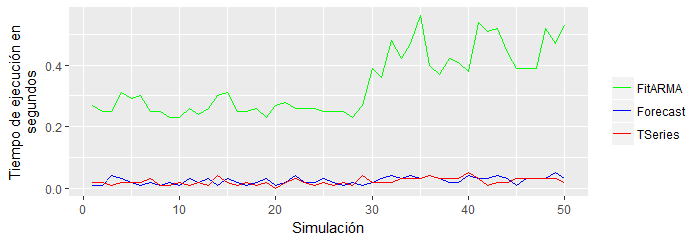
\includegraphics[scale = 0.7]{Images/Modelizacion/331.png}}
    \caption{Comparación de tiempos para los métodos de ajuste de modelos ARMA}
    \label{tiempos_modelos}
\end{figure}

\section{Opera Package}
Hasta ahora hemos utilizado modelos de distintas librerías para realizar predicciones sobre nuestra serie temporal. Lo que buscamos es optimizar el poder predictivo del modelo por lo que normalmente seleccionaremos aquel que nos ofrezca las predicciones más acertadas. Pero existen otros enfoques con los que podemos obtener mejores resultados.

Por la propia naturaleza de los distintos modelos tenemos que unos recogerán comportamientos indetectables por otros. Bajo estos supuestos tiene sentido combinar las predicciones de los distintos modelos a fin de intentar recoger toda la información posible. Una de las librerías encargada de implementar este tipo de técnicas es $\verb!opera!$ \cite{opera}. Se puede estudiar el código utilizado en este apartado en el Anexo IX.

Consideremos una serie de la forma $Y_1, Y_2,...,Y_t$. Hemos ajustado $K$ modelos cada uno de los cuales nos ofrece una predicción distinta para el tiempo $t+h$, a estas predicciones las denotaremos como $x_{k,t+h}$. Después calcularemos $\widehat{Y}_{t+h}$ combinando todas estas predicciones ponderando de acuerdo a su rendimiento, es decir:
\begin{equation}
    \widehat{Y}_{t+h} = \sum_{k = 1}^{K} p_{k,t+h} \enskip  x_{k,t+h}
\end{equation}

\noindent donde las ponderaciones $p_{k,t+h}$ se fijan de acuerdo al poder predictivo de los distintos modelos. Una de las principales características de este tipo de técnicas es que pueden implementarse en línea, es decir, pueden ir ajustando las ponderaciones a medida que se introducen nuevos valores del \textit{test}. Para entenderlo mejor a continuación se muestra el proceso que suelen seguir estas últimas:
\begin{enumerate*}
  \item Inicializamos las ponderaciones $p_{k,t+1}$ uniformemente.
  \item Calculamos las predicciones para el tiempo $t+1$ de los distintos K modelos ($x_{k,t+1}$).
  \item Calculamos $\widehat{Y}_{t+1}$ a partir de la suma ponderada de estas $K$ predicciones.
  \item Introducimos el valor real de la serie y ajustamos las ponderaciones de acuerdo a la función de pérdida definida.
  \item Estas ponderaciones ajustadas se denotan como $p_{k,t+2}$ y se utilizan para calcular $\widehat{Y}_{t+2}$.
  \item Se itera el proceso hasta que no tengamos más observaciones en nuestro conjunto de \textit{test}.
\end{enumerate*}

Este tipo de procesos son perfectos para modelos en los que la variable dependiente sigue una estructura temporal ya que este se puede ir actualizando a medida que tenemos nuevas observaciones de la serie.
\begin{figure}
    \centering
    \centerline{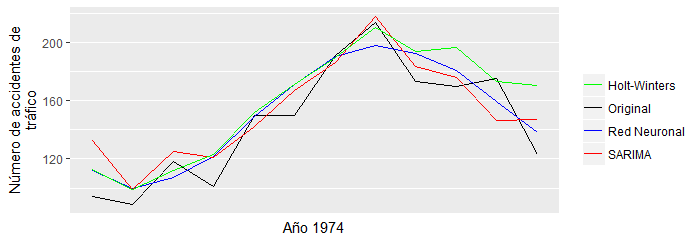
\includegraphics[scale = 0.7]{Images/Modelizacion/332.png}}
    \caption{Comparación del ajuste de los distintos modelos}
    \label{comp_entre_modelos}
\end{figure}

Vamos a combinar las predicciones a un año de tres modelos previamente ajustados: red neuronal, SARIMA$(1,0,0)(1,0,0)_{12}$ y triple suavizado de Holt-Winters. Sus respectivos MAE son de 13.27784, 14.86938 y 15.04762 y sus ajustes se muestran en la Figura \ref{comp_entre_modelos}. Para trabajar con los métodos de esta librería es necesario tener las predicciones de los tres modelos en un mismo objeto:
\begin{Verbatim}[fontsize=\footnotesize, numbers = left]
X <- cbind(red = pred.red$mean, sarima = pred.sarima$mean, hw = pred.hw$mean)
\end{Verbatim}

Es posible estudiar el error a nivel observacional gracias al método $\verb!loss()!$. Este método nos muestra el error cometido por cada uno de los tres modelos en cada observación del \textit{test}, su sintaxis es la siguiente:
\begin{Verbatim}[fontsize=\footnotesize]
loss(x, y, loss.type = "square")
\end{Verbatim}

A través de $\verb!x!$ se introducen las predicciones de los modelos, en $\verb!y!$ el conjunto de \textit{test} con el que se va a comparar y en $\verb!loss.type!$ el tipo de función de pérdida a utilizar.  Por defecto viene la cuadrática ($\verb!square!$) pero nosotros utilizaremos la absoluta ($\verb!absolute!$), que se corresponde con el MAE. En nuestro caso la salida resultante es la siguiente:
\begin{Verbatim}[fontsize=\footnotesize]
                          red    sarima        hw
          Jan 1974 18.0127432 38.527985 18.450649
          Feb 1974 10.9568480 10.320400  9.710105
          Mar 1974 11.0906385  7.150485  5.664850
          Apr 1974 20.4867823 19.718444 22.231049
          May 1974  0.6093056  7.863369  1.744073
          Jun 1974 21.3113668 17.094233 21.410794
          Jul 1974  0.7535920  4.476612  1.277397
          Aug 1974 15.9864688  3.778124  3.435301
          Sep 1974 19.4924576 10.727018 20.507963
          Oct 1974 10.5408218  6.081625 26.904985
          Nov 1974 15.2725507 28.796364  1.528908
          Dec 1974 14.7910821 23.897923 47.705347
\end{Verbatim}

Podemos apreciar como el MAE del SARIMA y el Holt-Winters parece mostrar un comportamiento irregular ya que intermensualmente varía mucho, sin embargo el MAE de la red neuronal parece mostrar un comportamiento más estable con variaciones más suaves.

\subsection{Combinaciones fuera de línea}
El método $\verb!oracle()!$ implementa una técnica para la combinación de predicciones no aplicable en línea ya que necesita desde un principio el conjunto de \textit{test} en su totalidad. Su sintaxis se muestra a continuación:
\begin{Verbatim}[fontsize=\footnotesize]
oracle(Y, experts, model = "convex", loss.type = "square",
       lambda = NULL, niter = NULL, ...)
\end{Verbatim}

En $\verb!Y!$ introducimos el conjunto de \textit{test} y en $\verb!experts!$ el objeto que contiene las predicciones realizadas por los tres modelos. A través de $\verb!model!$ especificaremos el tipo de combinación a utilizar, las principales opciones son las siguientes:
\begin{description}
  \item[$\bullet$ \PVerb{Expert}:]Selecciona las predicciones del modelo con mejor rendimiento.
  \item[$\bullet$ \PVerb{Convex}:]Selecciona la combinación convexa óptima para las distintas predicciones. Se cumple que para $\forall i \in K$:
  \begin{equation}
    p_{i,t+h} > 0
  \end{equation}
  \begin{equation}
    \sum_{i}^{} p_{i,t+h} = 1
  \end{equation}
  \item[$\bullet$ \PVerb{Linear}:]Selecciona la combinación lineal óptima para las distintas predicciones.
\end{description}

El argumento $\verb!loss.type!$ indica el tipo de función de pérdida a utilizar. El resto de argumentos ofrecen personalizaciones más complejas como la inclusión del parámetro de regularización para el caso lineal. Comenzaremos ajustando una combinación convexa con función de perdida absoluta. Para ello debemos escribir:
\begin{Verbatim}[fontsize=\footnotesize, numbers = left]
oracle.convex <- oracle(Y = acc.test, experts = X, loss.type = "absolute",
                        model = "convex")
\end{Verbatim}

Si aplicamos $\verb!plot()!$ al objeto generado por $\verb!oracle()!$ nos devuelve la Figura \ref{rendimiento}. En ella se muestra una comparativa del rendimiento predictivo de los tres modelos y sus combinaciones convexas y uniformes. Se puede apreciar que la combinación convexa es la que posee el MAE más bajo, seguida por la red neuronal y la combinación uniforme. El modelo SARIMA y el suavizado Holt-Winters son los que obtienen peores resultados. Para obtener las predicciones debemos recurrir al \textit{subsetting} $\verb!$predictions!$. En la Figura \ref{lin_conv} se muestra el ajuste generado por las nuevas predicciones.
\begin{figure}
    \centering
    \centerline{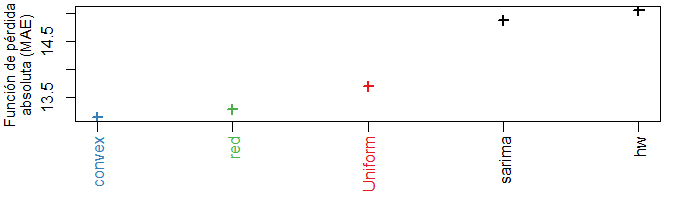
\includegraphics[scale = 0.7]{Images/Modelizacion/333.png}}
    \caption{Comparación del rendimiento entre modelos y combinaciones}
    \label{rendimiento}
\end{figure}

Vamos a hacer lo mismo solo que combinando linealmente las predicciones. Para ello pasaremos el argumento $\verb!model!$ como $\verb!linear!$. La comparativa del rendimiento se muestra en la Figura \ref{rendimiento_2}. Se puede apreciar como la combinación lineal es la que mejores resultados parece ofrecer, superando incluso a la convexa, sin embargo si estudiamos su ajuste en la Figura \ref{lin_conv} vemos que parece ajustarse muy bien en todo el conjunto de test menos en el pico correspondiente al mes de agosto. Aunque en este caso estamos obteniendo un MAE muy bajo la predicción no parece detectar este tipo de picos por lo que quizás no nos merecería la pena utilizarla.
\begin{figure}
    \centering
    \centerline{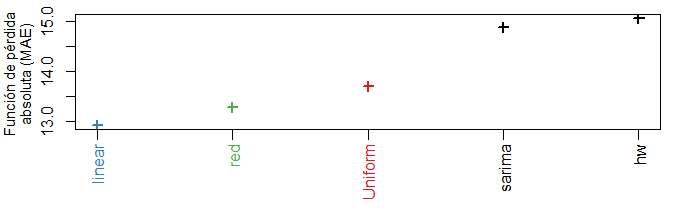
\includegraphics[scale = 0.7]{Images/Modelizacion/335.png}}
    \caption{Comparación del rendimiento entre modelos y combinaciones}
    \label{rendimiento_2}
\end{figure}

\begin{figure}
    \centering
    \centerline{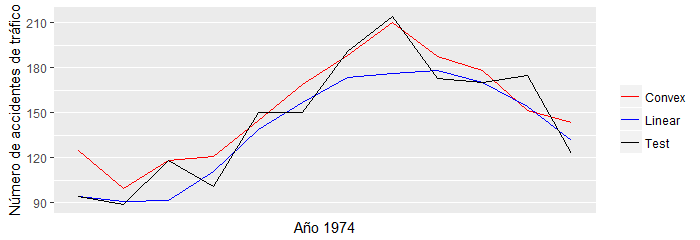
\includegraphics[scale = 0.7]{Images/Modelizacion/336337.png}}
    \caption{Ajuste de las combinaciones convexa y lineal al \textit{test}}
    \label{lin_conv}
\end{figure}

Este tipo de combinaciones nos permiten tener en cuenta a la hora de predecir los aspectos de varios modelos, sin embargo por la naturaleza de la estimación están limitados a trabajar con conjuntos de datos completos. Una posible forma de implementar esto en línea sería iterando la estimación de las ponderaciones con todo el conjunto de datos más las nuevas observaciones que fuesen entrando pero para sistemas grandes resultaría muy costoso computacionalmente, además de que se podría incurrir a problemas de índole estadística.

\subsection{Combinaciones en línea}
El método $\verb!mixture()!$ nos permite definir lo que se conocen como \textit{aggregation rules}. Este tipo de técnicas actualizan las ponderaciones secuencialmente permitiendo así el entrenamiento en línea. Su sintaxis es la siguiente:
\begin{Verbatim}[fontsize=\footnotesize]
mixture(Y = NULL, experts = NULL, model = "MLpol", loss.type = "square",
        loss.gradient = TRUE, coefficients = "Uniform", parameters = list())
\end{Verbatim}

A través de $\verb!Y!$ introducimos las observaciones del \textit{test}, en $\verb!experts!$ las predicciones realizadas por los modelos y en $\verb!loss.type!$ la función de pérdida sobre la que trabajaremos. El tipo de \textit{aggregation rule} a usar se define a través de $\verb!model!$. Hay varias opciones, algunas de ellas ponderan exponencialmente las predicciones respecto al tiempo, otras aplican algunas técnicas de optimización más complejas, etc…  El argumento $\verb!loss.gradient!$ hace que se trabaje sobre el gradiente de la función de pérdida mientras que $\verb!coefficients!$ determina los valores iniciales de las ponderaciones, por defecto viene como $\verb!Uniform!$ para no dar así prioridad a unos modelos sobre otros. Algunas de estas \textit{aggregation rules} dependen de ciertos parámetros que pueden ser clave para obtener unos resultados óptimos, el argumento $\verb!parameters!$ se encarga de controlarlos. Si se deja por defecto estima los parámetros secuencialmente, en caso contrario se le debe introducir valores para los parámetros y él seleccionará aquellos que ofrezcan un mejor resultado.

Lo más común es pasar los argumentos $\verb!Y!$ y $\verb!experts!$ vacíos ($\verb!NULL!$) haciendo que el método solo defina la estructura de la \textit{aggregation rule} a utilizar. Para predecir se utiliza $\verb!predict()!$ de la librería $\verb!opera!$. Su sintaxis se muestra a continuación.
\begin{Verbatim}[fontsize=\footnotesize]
predict(object, newexperts = NULL, newY = NULL,
        type = c("model", "response", "weights", "all"), ...)
\end{Verbatim}

A través de $\verb!object!$ se introduce el objeto definido por $\verb!mixture()!$, en $\verb!newexperts!$ y $\verb!newY!$ se va introduciendo secuencialmente las predicciones de los modelos y sus respectivos valores en el \textit{test}. El argumento $\verb!type!$ indica al método la salida que debe ofrecer. Recomiendo dejar este último por defecto para obtener todo de una vez.

Vamos a implementar una \textit{aggregation rule} con ponderaciones exponenciales en el tiempo ($\verb!EWA!$). El parámetro $\verb!eta!$ controlará  la rapidez con la que aprenderá de los valores del \textit{test} y de las estimaciones de los modelos, en este caso vamos a dejar que el método los estime internamente. Seguiremos trabajando con la función de pérdida absoluta e iniciaremos los coeficientes uniformemente. Primero iniciaremos la \textit{aggregation rule}:
\begin{Verbatim}[fontsize=\footnotesize, numbers = left]
mix <- mixture(model = "EWA", loss.type = "absolute", coefficients = "Uniform")
\end{Verbatim}

Después para hacerlo más intuitivo vamos a ir iterando observación a observación del \textit{test}. El código se muestra a continuación:
\begin{Verbatim}[fontsize=\footnotesize, numbers = left]
model <- mix
for (i in 1:length(as.vector(acc.test))) {
  model <- predict(model, X[i,], as.vector(acc.test)[i])
}
\end{Verbatim}

En cada iteración las ponderaciones se irán ajustando de acuerdo a la discrepancia entre las predicciones de los distintos modelos y la correspondiente observación del \textit{test}. De esta forma la \textit{aggregation rule} aprenderá de los errores cometidos por las predicciones y dará más importancia a unos modelos u otros. En nuestro caso solo hemos realizado 12 iteraciones. Si hacemos $\verb!print()!$ sobre el $\verb!model!$ resultante obtenemos lo siguiente:
\begin{Verbatim}[fontsize=\footnotesize]
          Aggregation rule: EWA
          Loss function:  absolute loss
          Gradient trick:  TRUE
          Coefficients:
          red   sarima      hw
            1 1.31e-05 4.2e-11
\end{Verbatim}

En este caso vemos que las ponderaciones finales para estos tres modelos son de 1 para la red neuronal y de prácticamente 0 para el SARIMA y el suavizado Holt-Winters. La \textit{aggregation rule} ha decidido dar todo el peso de la predicción a la red. Esto significa que si quisiésemos predecir el mes de enero de 1976 tendríamos que ponderar las predicciones de los tres modelos de esta forma. Con el \textit{subsseting} $\verb!$weights!$ vemos la evolución de las ponderaciones durante el proceso de estimación. En nuestro caso tenemos lo siguiente:
\begin{Verbatim}[fontsize=\footnotesize]
                     red       sarima        hw
          [1,] 0.3333333 3.333333e-01 0.3333333
          [2,] 0.6190265 7.268057e-10 0.3809735
          [3,] 0.4593810 3.786922e-02 0.5027498
          [4,] 0.3251488 3.166993e-01 0.3581519
          [5,] 0.3325841 3.319613e-01 0.3354546
          [6,] 0.3333720 3.327050e-01 0.3339230
          [7,] 0.3333242 3.332837e-01 0.3333921
          [8,] 0.3333340 3.333242e-01 0.3333418
          [9,] 0.3333317 3.333336e-01 0.3333347
         [10,] 0.3333331 3.333335e-01 0.3333334
         [11,] 0.3333333 3.333334e-01 0.3333333
         [12,] 0.3333333 3.333333e-01 0.3333333
\end{Verbatim}

Vemos que comienza con ponderaciones uniformes pero ya en la segunda iteración distribuye el peso entre la red y el suavizado dejando al SARIMA sin voz en la predicción. En la tercera da más peso al suavizado que a la red y sigue dejando al SARIMA casi en cero. Tras esto las ponderaciones parecen evolucionar uniformemente. En la Figura \ref{mix} se puede observar el ajuste de las predicciones ponderadas. En este caso estamos obteniendo un MAE de 14.07949.
\begin{figure}
    \centering
    \centerline{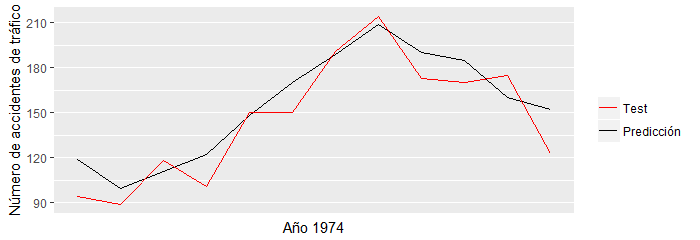
\includegraphics[scale = 0.7]{Images/Modelizacion/337.png}}
    \caption{Ajuste de las predicciones de \PVerb{mix} con el \textit{test}}
    \label{mix}
\end{figure}

Si le pasamos el método $\verb!plot()!$ al objeto $\verb!model!$ obtenemos varios gráficos muy interesantes (la salida completa se muestra en el Anexo X). En la Figura \ref{entre_modelos}  se muestra la comparativa del rendimiento de la combinación con los modelos individuales. Podemos apreciar como el mejor MAE lo tiene la red neuronal seguida por la combinación uniforme de predicciones y por la aggregation rule.

Este tipo de combinaciones funcionan bien para modelos cuyas predicciones correlacionen poco, ya que esto significa que cada uno está recogiendo una parte del proceso que genera los datos, sin embargo a veces consigue afinar las predicciones entre modelos correlacionados. En nuestro caso la red neuronal producía unas predicciones muy suavizadas y el SARIMA y suavizado Holt-Winters parecían mostrar más picos. Combinando las tres obtenemos una predicción que consigue aunar estas cualidades, mostrando un comportamiento suave con algunos picos en variaciones de la serie significativas. Además, estudiando las ponderaciones, podemos ver qué modelos poseen un mayor poder predictivo pudiendo así orientar nuestro tiempo y recursos a mejorarlos.
\begin{figure}
    \centering
    \centerline{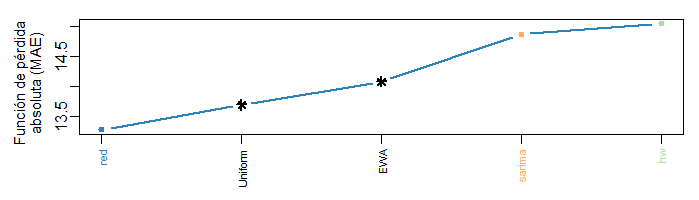
\includegraphics[scale = 0.7]{Images/Modelizacion/339.png}}
    \caption{{Comparación del rendimiento entre modelos, combinaciones y \PVerb{mix}}}
    \label{entre_modelos}
\end{figure}








